% CREATED BY DAVID FRISK, 2015

% IMPORT SETTINGS
\documentclass[11pt,a4paper,twoside]{report}
% CREATED BY DAVID FRISK, 2015

% BASIC SETTINGS
\usepackage{moreverb}								% List settings
\usepackage{textcomp}								% Fonts, symbols etc.
\usepackage{lmodern}								% Latin modern font
\usepackage{helvet}									% Enables font switching
\usepackage[T1]{fontenc}							% Output settings
\usepackage[english]{babel}							% Language settings
\usepackage[utf8]{inputenc}							% Input settings
\usepackage{amsmath}								% Mathematical expressions (American mathematical society)
\usepackage{amssymb}								% Mathematical symbols (American mathematical society)
\usepackage{graphicx}								% Figures
\usepackage{subfig}									% Enables subfigures
\numberwithin{equation}{chapter}					% Numbering order for equations
\numberwithin{figure}{chapter}						% Numbering order for figures
\numberwithin{table}{chapter}						% Numbering order for tables
\usepackage{listings}								% Enables source code listings
\usepackage{chemfig}								% Chemical structures
\usepackage[top=3cm, bottom=3cm,
			inner=3cm, outer=3cm]{geometry}			% Page margin lengths			
\usepackage{eso-pic}								% Create cover page background
\newcommand{\backgroundpic}[3]{
	\put(#1,#2){
	\parbox[b][\paperheight]{\paperwidth}{
	\centering
	\includegraphics[width=\paperwidth,height=\paperheight,keepaspectratio]{#3}}}}
\usepackage{float} 									% Enables object position enforcement using [H]
\usepackage{parskip}								% Enables vertical spaces correctly 



% OPTIONAL SETTINGS (DELETE OR COMMENT TO SUPRESS)

% Disable automatic indentation (equal to using \noindent)
\setlength{\parindent}{0cm}                         


% Caption settings (aligned left with bold name)
\usepackage[labelfont=bf, textfont=normal,
			justification=justified,
			singlelinecheck=false]{caption} 		

		  	
% Activate clickable links in table of contents  	
\usepackage{hyperref}								
\hypersetup{colorlinks, citecolor=black,
   		 	filecolor=black, linkcolor=black,
    		urlcolor=black}


% Define the number of section levels to be included in the t.o.c. and numbered	(3 is default)	
\setcounter{tocdepth}{5}							
\setcounter{secnumdepth}{5}	


% Chapter title settings
\usepackage{titlesec}		
\titleformat{\chapter}[display]
  {\Huge\bfseries\filcenter}
  {{\fontsize{50pt}{1em}\vspace{-4.2ex}\selectfont \textnormal{\thechapter}}}{1ex}{}[]


% Header and footer settings (Select TWOSIDE or ONESIDE layout below)
\usepackage{fancyhdr}								
\pagestyle{fancy}  
\renewcommand{\chaptermark}[1]{\markboth{\thechapter.\space#1}{}} 


% Select one-sided (1) or two-sided (2) page numbering
\def\layout{2}	% Choose 1 for one-sided or 2 for two-sided layout
% Conditional expression based on the layout choice
\ifnum\layout=2	% Two-sided
    \fancyhf{}			 						
	\fancyhead[LE,RO]{\nouppercase{ \leftmark}}
	\fancyfoot[LE,RO]{\thepage}
	\fancypagestyle{plain}{			% Redefine the plain page style
	\fancyhf{}
	\renewcommand{\headrulewidth}{0pt} 		
	\fancyfoot[LE,RO]{\thepage}}	
\else			% One-sided  	
  	\fancyhf{}					
	\fancyhead[C]{\nouppercase{ \leftmark}}
	\fancyfoot[C]{\thepage}
\fi


% Enable To-do notes
\usepackage[textsize=tiny]{todonotes}   % Include the option "disable" to hide all notes
\setlength{\marginparwidth}{2.5cm} 


% Supress warning from Texmaker about headheight
\setlength{\headheight}{15pt}		




\usepackage{graphicx}
\usepackage{lipsum,etoolbox}% http://ctan.org/pkg/{lipsum,etoolbox}
\usepackage{acro}
\usepackage[acronym]{glossaries}
\usepackage{amsmath,tabularx}
\usepackage{siunitx}
\usepackage[utf8]{inputenc}
\usepackage{nomencl}

\usepackage[svgnames]{xcolor}
\newcommand{\plogo}{\fbox{$\mathcal{PL}$}} % Generic dummy publisher logo

\usepackage[utf8]{inputenc} % Required for inputting international characters
\usepackage[T1]{fontenc} % Output font encoding for international characters
\usepackage{fouriernc} % Use the New Century Schoolbook font


\usepackage{listings}
\lstset{language=Fortran} 


\usepackage{listings}
\usepackage{color}

\definecolor{mygreen}{rgb}{0,0.6,0}
\definecolor{mygray}{rgb}{0.5,0.5,0.5}
\definecolor{mymauve}{rgb}{0.58,0,0.82}

\lstset{ %
  backgroundcolor=\color{white},   % choose the background color; you must add \usepackage{color} or \usepackage{xcolor}; should come as last argument
  basicstyle=\footnotesize,        % the size of the fonts that are used for the code
  breakatwhitespace=false,         % sets if automatic breaks should only happen at whitespace
  breaklines=true,                 % sets automatic line breaking
  captionpos=b,                    % sets the caption-position to bottom
  commentstyle=\color{mygreen},    % comment style
  deletekeywords={...},            % if you want to delete keywords from the given language
  escapeinside={\%*}{*)},          % if you want to add LaTeX within your code
  extendedchars=true,              % lets you use non-ASCII characters; for 8-bits encodings only, does not work with UTF-8
  frame=single,	                   % adds a frame around the code
  keepspaces=true,                 % keeps spaces in text, useful for keeping indentation of code (possibly needs columns=flexible)
  keywordstyle=\color{blue},       % keyword style
  language=Fortran,                 % the language of the code
  morekeywords={*,...},            % if you want to add more keywords to the set
  numbers=left,                    % where to put the line-numbers; possible values are (none, left, right)
  numbersep=5pt,                   % how far the line-numbers are from the code
  numberstyle=\tiny\color{mygray}, % the style that is used for the line-numbers
  rulecolor=\color{black},         % if not set, the frame-color may be changed on line-breaks within not-black text (e.g. comments (green here))
  showspaces=false,                % show spaces everywhere adding particular underscores; it overrides 'showstringspaces'
  showstringspaces=false,          % underline spaces within strings only
  showtabs=false,                  % show tabs within strings adding particular underscores
  stepnumber=1,                    % the step between two line-numbers. If it's 1, each line will be numbered
  stringstyle=\color{mymauve},     % string literal style
  tabsize=2,	                   % sets default tabsize to 2 spaces
  title=\lstname                   % show the filename of files included with \lstinputlisting; also try caption instead of title
}


 
\makenomenclature



\begin{document} 

% COVER PAGE, TITLE PAGE AND IMPRINT PAGE
\pagenumbering{roman}			% Roman numbering (starting with i (one)) until first main chapter
\begin{titlepage} % Suppresses headers and footers on the title page
	
	\centering % Centre everything on the title page
	
	%------------------------------------------------
	%	Top rules
	%------------------------------------------------
	
	\rule{\textwidth}{1pt} % Thick horizontal rule
	
	\vspace{2pt}\vspace{-\baselineskip} % Whitespace between rules
	
	\rule{\textwidth}{0.4pt} % Thin horizontal rule
	
	\vspace{0.1\textheight} % Whitespace between the top rules and title
	
	%------------------------------------------------
	%	Title
	%------------------------------------------------
	
	\textcolor{Red}{ % Red font color
		{\Huge Implementation of Laplace equation}\\[0.5\baselineskip] % Title line 1
		{\Large using}\\[0.5\baselineskip] % Title line 2
		{\Huge PETSc} % Title line 3
	}
	
	\vspace{0.025\textheight} % Whitespace between the title and short horizontal rule
	
	\rule{0.3\textwidth}{0.4pt} % Short horizontal rule under the title
	
	\vspace{0.1\textheight} % Whitespace between the thin horizontal rule and the author name
	
	%------------------------------------------------
	%	Author
	%------------------------------------------------
	
	{\Large \textsc{srikanth chowdadenahalli sathyanarayana}} % Author name
	
	\vfill % Whitespace between the author name and publisher
	
	%------------------------------------------------
	%	Publisher
	%------------------------------------------------
	
%	{\large\textcolor{Red}{\plogo}}\\[0.5\baselineskip] % Publisher logo
	
%	{\large\textsc{the publisher}} % Publisher
	
	\vspace{0.1\textheight} % Whitespace under the publisher text
	
	%------------------------------------------------
	%	Bottom rules
	%------------------------------------------------
	
	\rule{\textwidth}{0.4pt} % Thin horizontal rule
	
	\vspace{2pt}\vspace{-\baselineskip} % Whitespace between rules
	
	\rule{\textwidth}{1pt} % Thick horizontal rule
	
\end{titlepage}

%\newpage
%\restoregeometry
%\thispagestyle{empty}
%\mbox{}
% ABSTRACT

%\addcontentsline{toc}{chapter}{Abstract}
%% CREATED BY DAVID FRISK, 2015
%An Informative Headline describing the Content of the Report\\
%A Subtitle that can be Very Much Longer if Necessary\\
%NAME FAMILYNAME\\
%Department of Some Subject or Technology\\
%Chalmers University of Technology \setlength{\parskip}{0.5cm}

\thispagestyle{plain}            % Supress header 
\setlength{\parskip}{0pt plus 1.0pt}
\section*{Abstract}
\hspace{0.25cm}Grid distortion is usually one of the major problems in the field of Computational Fluid dynamics (CFD). The quality of the results obtained from the numerically modeled simulations hugely depends on grid quality. There are many instances in modeling a fluid dynamics problem where grid distortion is inevitable. When this occurs the corresponding Numerical Scheme used to approximate the fluxes must account for these opposing changes. \\
\\
\hspace{0.25cm}A new numerical scheme called the Preferred Direction Diffusion Scheme for the calculation of diffusive fluxes is presented in this thesis. The numerical scheme proposed here is less sensitive to grid quality, therefore, the transformation of the grids is expected to be more accurate compared to the traditional transformation techniques like central differencing.\\
\\
\hspace{0.25cm}Initially, the scheme is implemented in MATLAB to study its Mathematical behavior. It is further applied to an Unsteady heat Conduction equation in 3D. It is tested on a simple case-a Square duct with adverse grid conditions. The obtained results are compared with the results obtained from an existing numerical scheme with conventional transformation technique. Later, both the results are compared to an analytical solution and conclusions are drawn based on that. \\
\\
\hspace{0.25cm}The implemented scheme is further evaluated for its robustness and accuracy through appropriate code verification techniques. Code verification usually involves error evaluation of the numerical schemes for known benchmark results. The obvious choice for a benchmark solution is the analytical solution but it's usually impossible to obtain them with a sufficient solution structure. The method of Manufactured solutions (MMS) plays a useful role in this situation. This method is fairly straightforward and purely a mathematical procedure. \\
\\
\hspace{0.25cm}MMS is implemented in CALC++ for an unsteady heat equation in 3D and Navier-stokes equation. CALC++ is a massively parallel incompressible flow solver (written in C++) developed at the division of Fluid Dynamics, Chalmers University of Technology. The scheme is evaluated by subjecting it to systematic grid tests. Its performance is judged by studying the rate of reduction of the discretization error with increasing grid resolution.

% KEYWORDS (MAXIMUM 10 WORDS)
\vfill
Keywords: CFD, Numerical scheme, Diffusive fluxes, PDS, CD, MMS, CALC++, MATLAB .

\newpage                % Create empty back of side
\thispagestyle{empty}
\mbox{}
%\newpage
%\let\cleardoublepage\clearpage

%\newpage
%% CREATED BY DAVID FRISK, 2015
\thispagestyle{plain}			% Supress header
\section*{Acknowledgements}
Firstly, I would like to thank my parents and brother for supporting me in every way possible during my stay in Sweden. I would like to thank my supervisor Niklas Andersson for giving me an opportunity to work on this thesis. My understanding of numerical methods for fluid dynamics and programming vastly improved during the past year through this thesis. I am very grateful to him for that. I would also like to thank Ragnar Lárusson and Huadong Yao for helping me out with CALC++. Finally, I want to thank all my friends here in Gothenburg and back home.


\vspace{1.5cm}
\hfill
Srikanth, Gothenburg, November 2016

\newpage				% Create empty back of side
\thispagestyle{empty}
\mbox{}

%nomenclature
%
\renewcommand{\nomname}{List of Symbols}
%\renewcommand{\nompreamble}{The next list describes several symbols that will be later used within the body of the document}
 

\nomenclature{$T$}{temperature}
\nomenclature{$t$}{time}
\nomenclature{$\alpha$}{Thermal diffusivity}
\nomenclature{$(r,\Theta)$}{radial coordinates}
\nomenclature{$V$}{volume}
\nomenclature{$\overline{T}$}{cell averaged temperature}
\nomenclature{$S$}{arbitrary control surface}
\nomenclature{$A$}{cell face area}
\nomenclature{$(x_1,x_2,x_3)$}{Cartesian coordinates}
\nomenclature{$(\xi,\eta,\zeta)$}{Computational coordinates}
\nomenclature{$\Delta t$}{time step}
\nomenclature{$\mathcal{V}$}{cell properties}
\nomenclature{$\Psi$}{inverse components of preferred direction}

\section*{List of Symbols}
\noindent
\begin{tabularx}{\linewidth}{@{} l X @{}}
$T$  &  temperature \\
$t$  & time \\
$\alpha$  &  Thermal diffusivity\\
$(r,\Theta)$  &  radial coordinates \\
$V$    &  volume \\
$\overline{T}$  &  cell averaged temperature \\
$A$  &  cell face area \\
$(x_1,x_2,x_3)$  &  Cartesian coordinates\\
$(\xi,\eta,\zeta)$  &  Computational coordinates\\
$\Delta t$  &  time step\\
$\mathcal{V}$  &  cell properties\\
$\Psi$  &  Inverse components of preferred direction\\
$\varphi$  &  Flow variable\\
$\rho$ & density\\
$\nu$ & kinematic viscocity\\
$P$ & Pressure\\
$Q$ & unsteady term vector\\
$F$ & Flux vector\\


\end{tabularx}

\section*{Abbreviations}
\noindent
\begin{tabularx}{\linewidth}{@{} l X @{}}
$CFD$  & Computational Fluid Dynamics \\
$PDS$  &  Preferred direction Diffusion Scheme \\
$CD$  &  Central Differencing \\
$MMS$ & Method of Manufacured solutions\\
$OOA$ & Observed order of accuracy\\



\end{tabularx}



\makenomenclature
\newpage
\let\cleardoublepage\clearpage			% Create empty back of side
\thispagestyle{empty}
\mbox{}

%\input{include/front}

% TABLE OF CONTENTS
%\cleardoublepage
%\newpage
\tableofcontents
\let\cleardoublepage\clearpage


% START OF MAIN DOCUMENT
\cleardoublepage
\setcounter{page}{1}
\pagenumbering{arabic}			% Arabic numbering starting from 1 (one)
\setlength{\parskip}{0pt plus 1pt}

 %INTRODUCTION
% CREATED BY DAVID FRISK, 2015
\chapter{Introduction}
\hspace{0.25cm}Partially averaged Navier Stokes(PANS) is a growing variable resolution turbulence closure model. It has an ability to capture scales that vary from Direct numerical Simulations(DNS) and Reynolds Averaged Navier Stokes(RANS). The equations for PANS are obtained from the traditional RANS equations. A new parameter which is the ratio of unresolved turbulent quantities to the total turbulent quantities is defined in this method. This is the only the only term that differentiates PANS from RANS and DNS. The original RANS equations are converted to PANS using this parameter and the closure models are solved for the unresolved turbulent quantities. Therefore, lower value of this parameter directs PANS to DNS and the higher to RANS.\\


\hspace{0.25cm}In this age of computational fluid dynamics(CFD) where more accurate turbulence models are needed to capture complex flow patterns, there is a requirement of developing more accurate turbulence models and methods. RANS generally is not computationally expensive but it fails provide desired results. On the other hand, DNS provides almost exact results but at a huge computational cost. Therefore, there is a need for turbulence models which provide reasonable results for realistic computational resources. PANS tries to achieve that\cite{giri}.\\



\hspace{0.25cm}This report presents the implementation of PANS for k-$\omega$ SST turbulence model in OpenFOAM. This implementation is initially described through governing equations. Further, it is tested on a Surface mounted cube case. The further section describes the geometry and different grids used for this case. A description of the boundary conditions and numerical schemes is also given in this section. Finally, the results obtained for several cases is presented. A comparison of the obtained results with the experimental plots is presented.




%% CREATED BY DAVID FRISK, 2015

\chapter{Governing Equations and Solution methods}

\section{Governing Equations}
\subsection{Laplace equation}The Laplace equation in 2D solved in this code is given below,
\begin{equation}\label{eq:uhe}
 \frac{\partial^2 T}{\partial x^2}+\frac{\partial^2 T}{\partial y^2} = 0
\end{equation}

$T$ is any physical variable like Temperature etc., and $x$ and $t$ represent the spatial coordinates.







\section{Numerical Method}
\hspace{0.25cm}The governing equation can be discretised using finite difference method and the final equation is expressed below. 

A standard 5 point stencil is represented by, 
\begin{figure}[H]
\centering
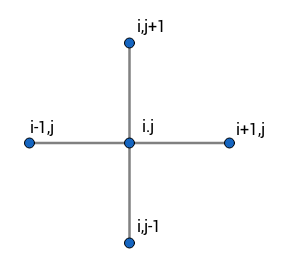
\includegraphics[scale=0.4]{figures/stencil.png}
\caption{five point stencil}
\label{fig:rline}
\end{figure}
Using the above representation, the final equation can be written as,
\begin{equation}
         T_{i,j}+\frac{1}{4}(T_{i,j+1}+T_{i,j-1}+T_{i,j+1}+T_{i,j-1}) 
\end{equation}


    




%\chapter{Preferred Direction Diffusion Scheme}
\label{chap:pdds}
\begin{figure}[h]
\centering
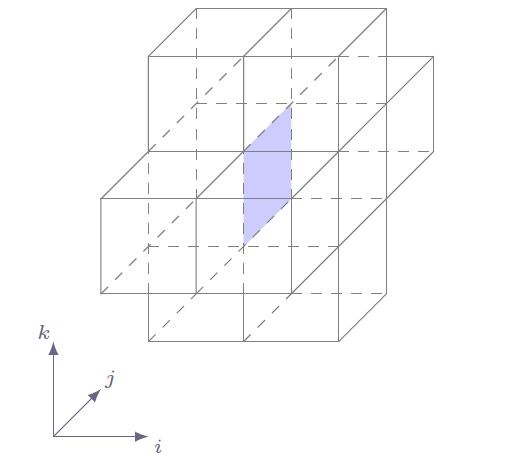
\includegraphics{figure/governing/fluxmolecule.JPG}
\caption{Representation of Flux Molecule in Computational Space}
\label{fig:fm}
\end{figure}
\hspace{0.25cm}In this new numerical scheme, the diffusion gradients on the faces are evaluated using the cell averages obtained from the surrounding ten cells as indicated in figure (\ref{fig:fm}). Note that, since the faces near domain boundaries are not surrounded by ten cells, they have to be treated differently. Twenty cell properties including volume of the cell are calculated for each of the considered ten cells per face in the physical space (\ref{sec:one}). These volume integrals are calculated using Gauss-point Quadrature (\ref{sec:gpq}).
\section{Preferred Direction}
\begin{figure}[h]
\centering
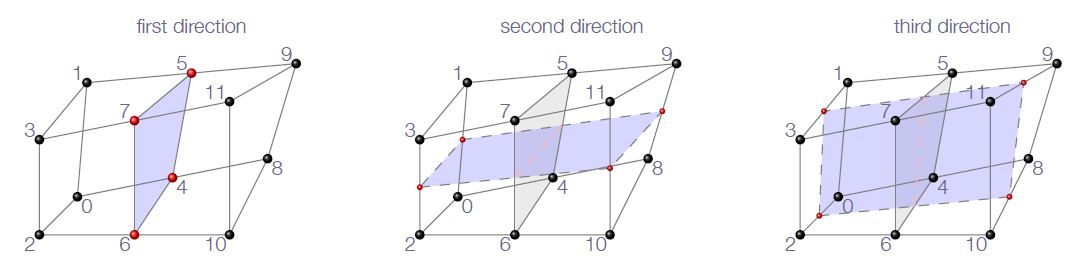
\includegraphics[width=1\linewidth]{figure/governing/pd.JPG}
\caption{Preferred Directions of a face}
\label{fig:pd}
\end{figure}
\hspace{0.25cm} In order to calculate the gradient coefficients for each face, three unique directions for each face inside the domain is calculated. Three planes are defined using the grid nodes. These directions are referred to as preferred directions, see figure (\ref{fig:pd})
      
     The preferred directions for each face of the flux molecule are calculated using the following relations,
     \begin{equation}
     \label{eq:pdeq}
         \begin{gathered}
         $First direction$,\hspace{1cm} n1=\frac{(r_7-r_4)\times(r_5-r_6)}{|(r_7-r_4)\times(r_5-r_6)|}\\
         $Second direction$,\hspace{1cm} n2=\frac{(r_{10}-r_0)\times(r_8-r_2)+(r_{11}-r_1)\times(r_9-r_3)}{|(r_{10}-r_0)\times(r_8-r_2)+(r_{11}-r_1)\times(r_9-r_3)|}\\
         $Third direction$,\hspace{1cm} n3=\frac{(r_9-r_0)\times(r_8-r_1)+(r_{11}-r_2)\times(r_{10}-r_3)}{|(r_9-r_0)\times(r_8-r_1)+(r_{11}-r_2)\times(r_{10}-r_3)|}
         \end{gathered}
     \end{equation}
The directions $n1$, $n2$ and $n3$ are not in general normal to each other.

\section{Local Co-ordinates}
    \label{sec:lc}
  \hspace{0.25cm}  A local co-ordinate system is now established for each face using the directions obtained in equation (\ref{eq:pdeq}). This co-ordinate system relates the global co-ordinate system, the preferred directions and the reference point $(x_o,y_o,z_o)$ located at the face center. 
    \begin{equation}
    \begin{gathered}
    \label{eq:lcs}
    \begin{bmatrix}
    x\\
    y\\
    z
    \end{bmatrix}= \begin{bmatrix}
    x_o\\
    y_o\\
    z_o
    \end{bmatrix}+\xi \begin{bmatrix}
    n1_x\\
    n1_y\\
    n1_z
    \end{bmatrix}+\eta\begin{bmatrix}
    n2_x\\
    n2_y\\
    n2_z
    \end{bmatrix}+\zeta\begin{bmatrix}
    n3_x\\
    n3_y\\
    n3_z\\
    \end{bmatrix}\\
    \begin{bmatrix}
    n1_x & n2_x & n3_x\\
    n1_y & n2_y & n3_y\\
    n1_z & n2_z & n3_z\\
    \end{bmatrix} 
    \begin{bmatrix}
    \xi\\
    \eta\\
    \zeta\\
    \end{bmatrix}=N\begin{bmatrix}
    \xi\\
    \eta\\
    \zeta\\
    \end{bmatrix}=\begin{bmatrix}
    x-x_o\\
    y-y_o\\
    z-z_0\\
    \end{bmatrix}\\
    \begin{bmatrix}
    \xi\\
    \eta\\
    \zeta\\
    \end{bmatrix}=N^{-1}\begin{bmatrix}
    x-x_o\\
    y-y_o\\
    z-z_0\\
    \end{bmatrix}\\
    \begin{bmatrix}
    \xi\\
    \eta\\
    \zeta\\
    \end{bmatrix}=\begin{bmatrix}
    \Psi_{11} & \Psi_{12} & \Psi_{13}\\
    \Psi_{21} & \Psi_{22} & \Psi_{23}\\
    \Psi_{31} & \Psi_{32} & \Psi_{33}\\
    \end{bmatrix}
    \begin{bmatrix}
    x-x_o\\
    y-y_o\\
    z-z_0\\
    \end{bmatrix}
    \end{gathered}
    \end{equation}
    
\section{Extraction of Gradient Coefficients}
\hspace{0.25cm}The variation of the flow variable $\varphi$ in the computational space, $(\xi,\eta,\zeta)$ is assumed to be,
\begin{equation}\label{eq:nmnm}
    {\varphi}(\xi,\eta,\zeta)=C_0+C_1\xi+C_2\eta+C_3\zeta+C_4\xi\eta+C_5\xi\zeta+C_6\eta^2+C_7\zeta^2+C_8\xi\eta^2+C_9\xi\zeta^2
\end{equation}

The unknown coefficients $[C_0....C_9]$ are obtained by solving a system of equations obtained by integrating the equation (\ref{eq:nmnm}) over the ten cell volumes of a Flux molecule (see figure \ref{fig:fm}).

\begin{equation}
\label{eq:big}
\begin{gathered}
    \begin{bmatrix}
    \overline{\varphi}_0 V_0 &.&.&.&
    \overline{\varphi}_9 V_9 
    \end{bmatrix}=\begin{bmatrix}
    C_0 &.&.&.&
    C_9
    \end{bmatrix}\begin{bmatrix}
    \int\int\int_{\Omega_0}\,d\Omega& \cdots \int\int\int_{\Omega_0} \xi\zeta^2 d\,\Omega \\
    .   &                                                                        .\\
    .    &                                                                        .\\
    .     &                                                                          .\\
    \int\int\int_{\Omega_9}\,d\Omega& \cdots \int\int\int_{\Omega_9} \xi\zeta^2 d\,\Omega \\
    \end{bmatrix}\\
    $Or$\\
    {\Phi}=\begin{bmatrix}
    C_0 &.&.&.&
    C_9
    \end{bmatrix} A
    \end{gathered}
\end{equation}
In equation (\ref{eq:big}), $\Phi$ represents the degrees of freedom in the CFD solver (cell-averages of the considered solver variables). Since the vector $\Phi$ is known the matrix $A$ can be calculated from the known metric data obtained in equations (\ref{eq:eqns} and \ref{eq:lcs}). Thus, the vector $\Phi$ can be represented as,
\begin{equation}
    \begin{bmatrix}
    C_0&.&.&.&C_9
    \end{bmatrix}=\Phi A^{-1}
\end{equation}
A detailed derivation of the integrals in the $A$ matrix is provided in Appendix \ref{app:aa}. Also, the procedure for obtaining the integrals in the domain boundaries is provided.

\section{Face Gradients}
\hspace{0.25cm}Further, differentiating equation (\ref{eq:nmnm}),
\begin{equation}
\label{eq:a18}
\begin{gathered}
    {d\varphi}=C_1d\xi+C_2d\eta+C_3d\zeta+C_4\xi d\eta+C_4\eta d\xi+C_5 \xi d\zeta+C_5 \zeta d\xi+\\
    2C_6\eta d\eta+2C_7\zeta d\zeta+C_8 \xi \eta d\eta+C_8 \eta^2 d\xi+2C_9\xi\zeta d\zeta+C_9\zeta^2 d\xi
\end{gathered}
\end{equation}
Since the local coordinate system is centered at the face center, equation (\ref{eq:a18}) results in,
\begin{equation}
    \label{eq:a19}
    \begin{gathered}
    (\xi,\eta,\zeta)=(0,0,0)\\
    {d\varphi}=C_1d\xi+C_2d\eta+C_3d\zeta
    \end{gathered}
\end{equation}
By Differentiating the second equation in (\ref{eq:lcs}), the relationship between the derivatives in ($x$,$y$,$z$) space and ($\xi$,$\eta$,$\zeta$) space is obtained as,
\begin{equation}
    \label{eq:a20}
    \begin{gathered}
    \begin{bmatrix}
    dx\\
    dy\\
    dz\\
    \end{bmatrix}=\begin{bmatrix}
    n1_x&n2_x&n3_x\\
    n1_y&n2_y&n3_y\\
    n1_z&n2_z&n3_z\\
    \end{bmatrix} \begin{bmatrix}
    d\xi\\
    d\eta\\
    d\zeta\\
    \end{bmatrix}=N \begin{bmatrix}
     d\xi\\
    d\eta\\
    d\zeta\\
    \end{bmatrix}
    \end{gathered} 
\end{equation}
Finally, the equations in (\ref{eq:a19} and \ref{eq:a20}) are combined to obtain the coefficients required for calculating the derivatives of ${\varphi}$ in the Cartesian coordinate system ($x$,$y$,$z$) at the face center.
\begin{equation}
    \label{eq:a21}
    \begin{gathered}
    \begin{bmatrix}
    Cx_0\\
    .\\
    .\\
    .\\
    Cx_9\\ \end{bmatrix}= \begin{bmatrix}
    (n1_xA^{-1}_{10}+n2_xA^{-1}_{20}+n3_xA^{-1}_{30})V_0\\
    \cdot\\
    \cdot\\
    \cdot\\
    (n1_xA^{-1}_{19}+n2_xA^{-1}_{29}+n3_xA^{-1}_{39})V_9\\
    \end{bmatrix}\\
     \begin{bmatrix}
    Cy_0\\
    .\\
    .\\
    .\\
    Cy_9\\ \end{bmatrix}= \begin{bmatrix}
    (n1_yA^{-1}_{10}+n2_yA^{-1}_{20}+n3_yA^{-1}_{30})V_0\\
    \cdot\\
    \cdot\\
    \cdot\\
    (n1_yA^{-1}_{19}+n2_yA^{-1}_{29}+n3_yA^{-1}_{39})V_9\\
    \end{bmatrix}\\
     \begin{bmatrix}
    Cz_0\\
    .\\
    .\\
    .\\
    Cz_9\\ \end{bmatrix}= \begin{bmatrix}
    (n1_zA^{-1}_{10}+n2_zA^{-1}_{20}+n3_zA^{-1}_{30})V_0\\
    \cdot\\
    \cdot\\
    \cdot\\
    (n1_zA^{-1}_{19}+n2_zA^{-1}_{29}+n3_zA^{-1}_{39})V_9\\
    \end{bmatrix}\\
    \\
    \\
     \frac{\partial {\varphi}}{\partial x} = \begin{bmatrix}
    Cx_0....Cx_9
    \end{bmatrix} \begin{bmatrix}
    \overline{{\varphi}_0}\\
   \cdot\\
    \cdot\\
    \cdot\\
    \overline{{\varphi}_9}
    \end{bmatrix},
    \frac{\partial {\varphi}}{\partial y} = \begin{bmatrix}
    Cy_0....Cy_9
    \end{bmatrix} \begin{bmatrix}
    \overline{{\varphi}_0}\\
    \cdot\\
    \cdot\\
    \cdot\\
    \overline{{\varphi}_9}
    \end{bmatrix},
    \frac{\partial {\varphi}}{\partial z} = \begin{bmatrix}
    Cz_0....Cz_9
    \end{bmatrix} \begin{bmatrix}
    \overline{{\varphi}_0}\\
   \cdot\\
    \cdot\\
    \cdot\\
    \overline{{\varphi}_9}
    \end{bmatrix}
    \end{gathered}
\end{equation}




%\chapter{Method of Manufactured Solutions (MMS)}
\label{ch:mmsd}
\hspace{0.25cm}Method of Manufactured solutions is one of the most sophisticated code verification methods available in the field of computational science and engineering \cite{codemms}. The main idea behind this method is to manufacture a solution for a flow variable using a continuous function instead of obtaining an exact solution. This manufactured solution need not be physically realistic since code verification is purely a mathematical procedure. Using the manufactured solution a source term is derived for the governing equation. Now, this governing equation is solved using numerical methods and compared with the existing known manufactured solution. Therefore, this method could also be seen as a problem solved backward. \\
For example, consider a function,
\begin{equation}\label{41}
    F(a)=0
\end{equation}
Now, say $a=u$ in (\ref{41}),
\begin{equation}\label{42}
    F(u)\neq0
\end{equation}
It is not necessary for $u$ to be a solution for (\ref{41}), therefore consider (\ref{42}) to be equal to a source term $Q$,
\begin{equation}\label{442}
    F(u)=Q
\end{equation}
\begin{equation}\label{43}
    F(a)=Q
\end{equation}
Now, $a=u$ is a solution for (\ref{43}). This is the fundamental idea behind the method of manufactured solutions.
\section{General procedure of MMS}
\hspace{0.25cm}The following steps are used to obtain the observed order of accuracy required to verify the code,
\\


\begin{equation}
\frac{\partial (\rho k_u)}{\partial t}+\frac{\partial (\rho k_u <V_j>)}{\partial x_j}=P_k-\beta^*k_u w_u+\frac{\partial}{\partial x_j}(\Gamma_{k_u}\frac{\partial k_u}{\partial x_j})
\end{equation}
\begin{equation}
\begin{split}
\frac{\partial (\rho \omega_u)}{\partial t}+\frac{\partial (\rho \omega_u <V_j>)}{\partial x_j}=\frac{\gamma}{\nu_u}P_k-(\frac{1}{f_\omega}-1)\frac{\gamma\beta^*}{\nu_u}\omega_uk_u-\\\frac{\beta\rho\omega_u^2}{f_\omega}+(1-F_{1u})2\rho\sigma_{w2}\frac{f_\omega}{f_k}\frac{1}{\omega_u}\frac{\partial k_u}{\partial x_j}\frac{\partial \omega_u}{\partial x_j}+\frac{\partial}{\partial x_j}(\Gamma_{\omega_u}\frac{\partial \omega_u}{\partial x_j})
\end{split}
\end{equation}
\begin{itemize}
  \item Determine the governing equations.
  \item Construct a manufactured solution.
  \item Use the solution to compute the source term to modify the governing equations.
  \item Obtain initial and boundary conditions using the manufactured solution.
  \item Setup a case by obtaining a grid to the domain and define suitable parameters like time step etc.
  \item Perform simulations for the modified equations on multiple mesh levels.
  \item Obtain the global discretization error of the numerical solutions.
  \item Conduct the order of accuracy test using the solution to determine if the observed order of accuracy matches the formal order of accuracy.
\end{itemize}
\newpage
An example of MMS using 1D unsteady heat equation is provided in appendix \ref{app=mms}.
\section{Manufactured Solutions}
\hspace{0.25cm}To ensure the accuracy of the code verification procedure special care has to be taken to obtain the manufactured solution. Some of them are mentioned below,\\
\begin{itemize}
  \item The considered manufactured solution should contain smooth analytic functions which ensure that the obtained solution will match the formal order of accuracy.
  \item The solution should have a sufficient number of non-trivial derivatives. For example, in momentum equation, if the manufactured solution for velocity is linear and if the diffusion term is solved using a second-order method, it would lead to incorrect predictions of the observed order of accuracy.
  \item The manufactured solution derivatives should be bounded by a constant to ensure that the solution is not varying strongly in space and time. Also, this ensures that the solution does not contain any singularities.
  \item The chosen solution should be realistic when pertaining to a particular flow variable. For example, if the physics of the problem demands positive temperature, the obtained manufactured solution must be compatible.\\
\end{itemize} 
The following are the manufactured solutions used in this thesis,
\begin{equation}\label{eq:44}
\begin{gathered}
    T(x,y,z,t)=e^{4\pi^2t}cos^2(2\pi x)cos^2(2\pi y)cos^2(2\pi z)\\
    u(x,y,z,t)=((0.5cos(\pi x)cos(\pi y)cos(\pi z)cos(\pi t))+0.5)\\
    v(x,y,z,t)=((0.25sin(\pi x)sin(\pi y)cos(\pi z)cos(\pi t))+0.5)\\
    w(x,y,z,t)=((0.25sin(\pi x)cos(\pi y)sin(\pi z)cos(\pi t))+0.5)\\
    p(x,y,z,t)=((cos(\pi x)cos(\pi y)cos(\pi z)cos(\pi t))+0.5)\\
\end{gathered}
\end{equation}
The velocity solutions are obtained in a way as to satisfy the continuity equation. 
\section{Initial and boundary conditions}
\hspace{0.25cm}Initial solution is obtained using the manufactured solutions in (\ref{eq:44}). A solution for a differential equation can be obtained using different types of boundary conditions. Using this principle, the boundary values are obtained from the manufactured solutions. For example, consider a case where the code obtains a solution using Dirichlet boundary condition on one of the boundary faces. This implementation can be directly performed and compared using the manufactured solutions. If the same solution is required using a Neumann condition on the same face, the values can be directly obtained from the derivatives of the manufactured solutions. 
\section{Discretization error}
\hspace{0.25cm}The normalized global discretization error of the obtained numerical solution and manufactured solution is obtained by employing $L_2$ norm,\\
\begin{equation}
\begin{gathered}
\label{eq:l2norm}
L_{2,i}=\Big(\frac{\sum_{n=1}^{N}|f_{i,n}-f_{exact,n}|^2}{N}\Big)^{1/2}
\end{gathered}
\end{equation}
Here, $i$ is for a particular mesh level.
\newpage
\section{Strengths and Limitations of MMS}
Some of the strengths of MMS are,\\
\begin{itemize}
  \item Most of the coding options can be verified using this method.
  \item It has the capability to handle nonlinear and coupled equations.
  \item It can be used to detect mistakes in the solution algorithm.
  \item It works equally well for finite difference, finite volume and finite element schemes.
\end{itemize} 
\vspace{0.4cm}
Some of the limitations are,\\
\begin{itemize}
  \item It is required to change the source code in order to accommodate the changes in the governing equations. The changes include the source term, initial, and boundary condition terms. Therefore, this process cannot be conducted as a black box analysis.
  \item To test other model options in the code, it's required to change the source term which can be time-consuming.
  \item The solutions are assumed to be smooth in the domain. Therefore, it is challenging to obtain manufactured solutions in cases involving discontinuities (shock waves, etc.).
\end{itemize}
\begin{comment}
\section{Grid configurations for MMS}
The main objective of using this method in this project is to test the robustness and accuracy of the numerical scheme with different mesh qualities. To achieve this, a set of systematically refined grids are generated and  in each case, the code will be tested. This test is further conducted for several grid configurations which involve skewness, non-orthogonality, and curvature (see figure ). 
\subsection{Non-orthogonality}
\subsection{Grid skewness}

\section{Observed order of accuracy}
\end{comment}






% CREATED BY DAVID FRISK, 2015
\chapter{Implementation}

\section{My learning}
\begin{itemize}
  
  
 
\end{itemize}

\section{Petsc learning}

\begin{itemize}
  \item Perform standard installation.
  \item dont forget to link the environment.
  \item read the manual.
  \item go through all the tutorial examples.
  
 
\end{itemize}





% THEORY
% CREATED BY DAVID FRISK, 2015
\chapter{Directions to use the code}
\section{General instructions}
The following points directs the user on how to compile and use the 1D Fortran code.
\\

\begin{itemize}
  \item Unzip the folder contents.
  \item The user must have already installed Fortran and Python compilers.
  \item Consult the Makefile for general compiling information.
  \item Type "make clean" to remove any already compiled files.
  \item Open "global.f95" file.
  \item Enter the details required to set up the case in that particular file.
  \item Type "make" to compile.
  \item Type "./heat" to execute the case.
  \item Text files are generated in the same folder.
  \item To post process, type "make output\_script.py".
  \item A list of text files available to post process is generated in the terminal.
  \item Choose for which time the user wants to display the plot.
  \item Type that particular time(the entire number) without the .txt extension.
  \item The plot is saved in the folder which can be viewed.
  \item To view another plot type "yes" and enter the time.
  \item To run another case with the compiled code type "make remove", make the changes in the global file and then type "make.
  \item To view the MMS results, change the value in the global file to "1"
  \item MMS results can be directly compared with the analytical results(for MMS) in the terminal.
\end{itemize}

\section{To note}

\begin{itemize}
  \item The code has some minor bugs but it should work as long as the stability criterion for explicit Euler is met.
  \item MMS is showing stability issues with the code which is natural due to the usage of explicit Euler. 
  \item For this reason, more work has to be done to better the MMS implementation but the working can be generally understood.
  \item It has to be considered that this a very small implementation and a base for improving it's efficiency. 
  
  
\end{itemize}



% METHODS

% RESULTS
%% CREATED BY DAVID FRISK, 2015
\chapter{Results }

\hspace{0.25cm}This section explores the computational results obtained from the implementation. An explanation of the results is attempted and further comparison plots with the experimental results is provided.The experimental results were obtained from \cite{exp}.The main objective of this section is provide plots to show the behaviour of PANS with changing $f_k$(input).


\hspace{0.25cm}Initially RANS simulations were performed on the same geometry and grid to get an idea of the lower limit of$f_k$. Based on that, a set of $f_k$ values were chosen for both coarse and fine grids. The results obtained from them is reported in this section. A contour plot of mean and instantaneous Velocities is first shown. Further, $f_k$(output) comparison contour plots are displayed. A comparison line plots comparing several mean quantities with the experimental values is provided later.

\hspace{0.25cm}The simulations were monitored by measuring the drag fluctuations around the cube. Figure \ref{fig:41} represents plots of such fluctuations. It can be observed that for a coarse grid with $f_k$=0.8, the fluctuations normalize after sometime and it just captures the vortex shedding(RANS behaviour). Contrary to that, with $f_k$=0.15 for a fine grid, it shows that PANS can also capture further fluctuations along with vortex shedding.

\begin{figure}[H]
\begin{minipage}[b]{0.5\linewidth}
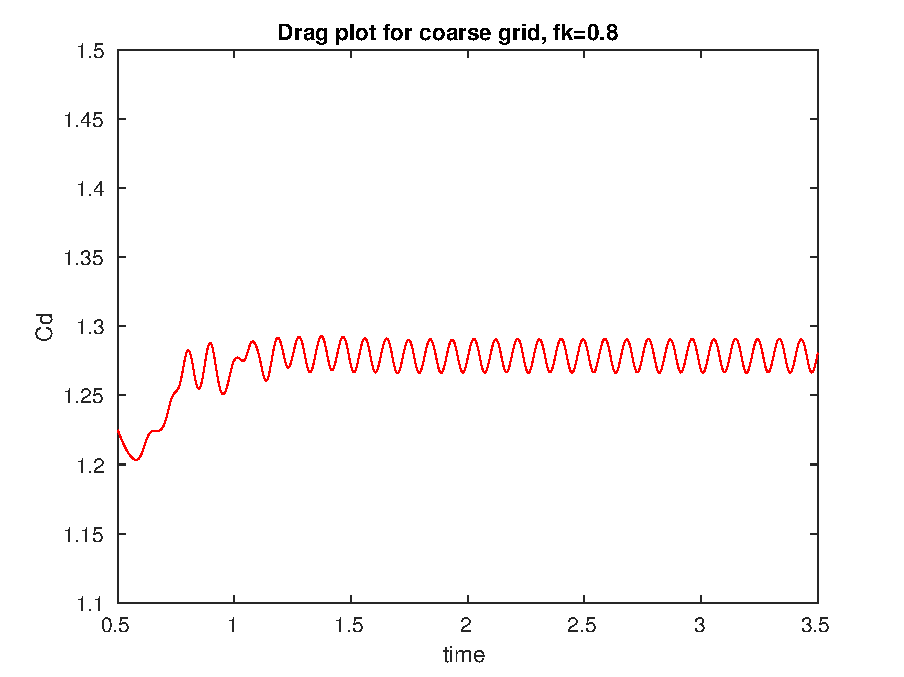
\includegraphics[scale=0.5]{figure/coarse/cd_coarse.pdf}
\end{minipage}
\begin{minipage}[b]{0.5\linewidth}
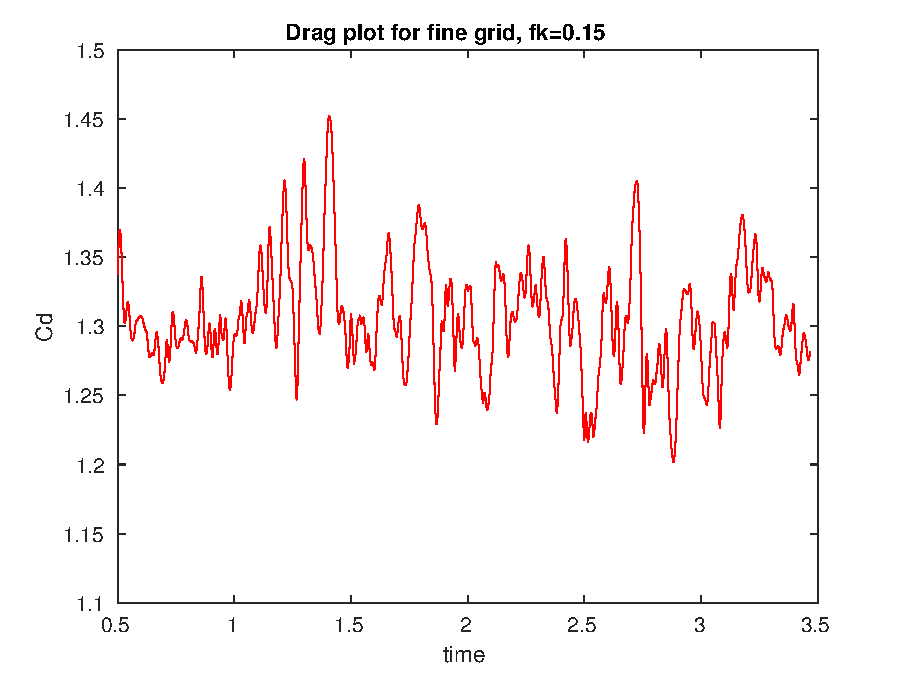
\includegraphics[scale=0.5]{figure/fine/cd_fine.pdf}
\end{minipage}
\caption{Drag fluctuations around the cube for coarse(left) and fine(right) grids}
\label{fig:41}
\end{figure}



\section{Mean Velocity Contour plots}

Figures \ref{fig:42} and \ref{fig:43} show the mean velocity plots along x direction for both coarse and fine grids. The simulations were averaged over 6 flow passes. The contour plots were obtained along the mid plane of the geometry. 


\begin{figure}[H]
\begin{minipage}[b]{0.5\linewidth}
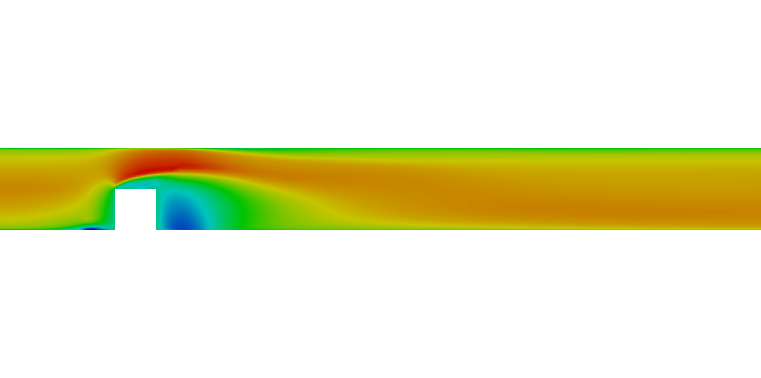
\includegraphics[scale=0.25]{figure/coarse/eight/Umean_z.png}
\caption*{$f_k$=0.8}
\end{minipage}
\begin{minipage}[b]{0.5\linewidth}
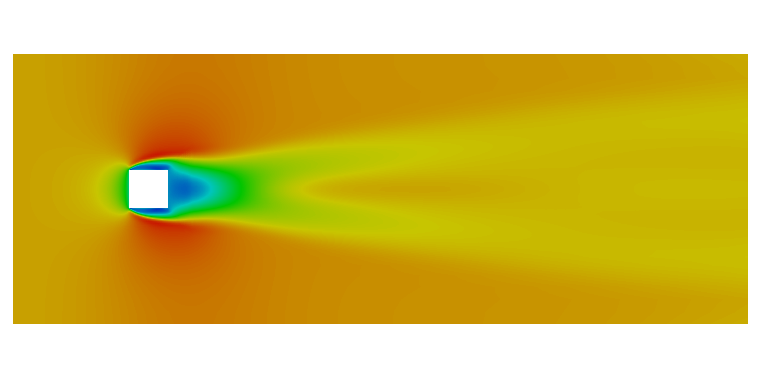
\includegraphics[scale=0.25]{figure/coarse/eight/Umean_y.png}
\caption*{}
\end{minipage}\\
\begin{minipage}[b]{0.5\linewidth}
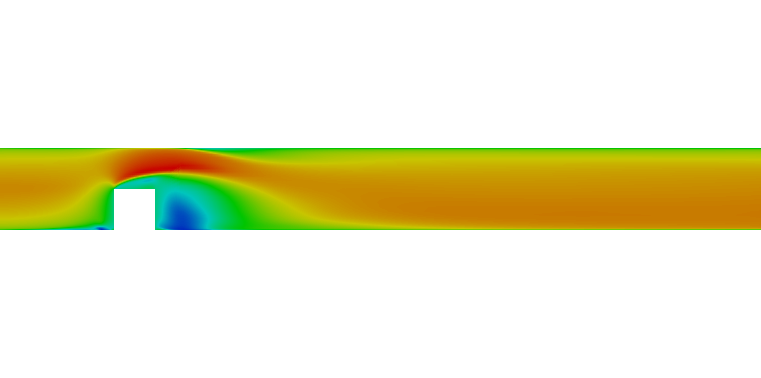
\includegraphics[scale=0.25]{figure/coarse/three/Umean_z.png}
\caption*{$f_k$=0.3}
\end{minipage}
\begin{minipage}[b]{0.5\linewidth}
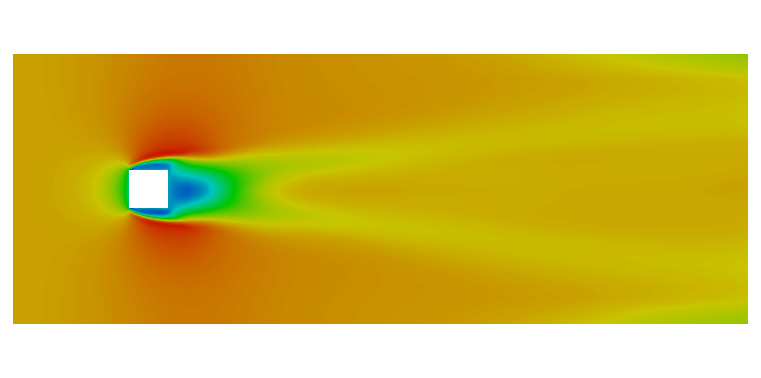
\includegraphics[scale=0.25]{figure/coarse/three/Umean_y.png}
\caption*{}
\end{minipage}\\
\begin{minipage}[b]{0.5\linewidth}
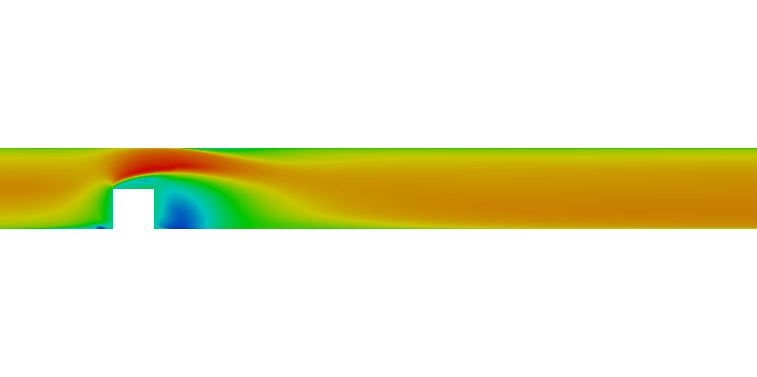
\includegraphics[scale=0.25]{figure/coarse/two/Umean_z.png}
\caption*{$f_k$=0.2}
\end{minipage}
\begin{minipage}[b]{0.5\linewidth}
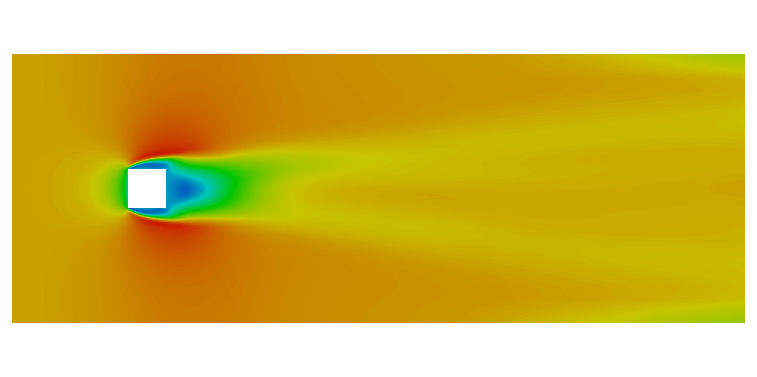
\includegraphics[scale=0.25]{figure/coarse/two/Umean_y.png}
\caption*{}
\end{minipage}\\
\begin{minipage}[b]{0.5\linewidth}
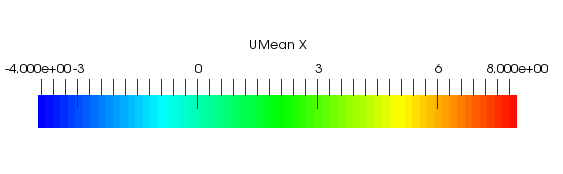
\includegraphics[scale=0.35]{figure/z_scale.png}
\end{minipage}
\begin{minipage}[b]{0.5\linewidth}
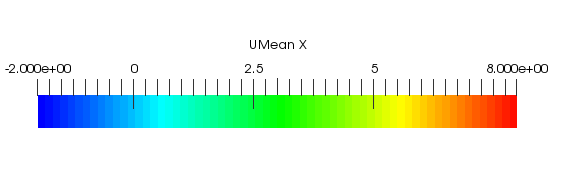
\includegraphics[scale=0.35]{figure/y_scale.png}
\end{minipage}\\

\caption{Mean velocity(U) plots about Z axis(left) and Y axis(right) for coarse grid}
\label{fig:42}
\end{figure}
\hspace{0.25cm}





\begin{figure}[H]
\begin{minipage}[b]{0.5\linewidth}
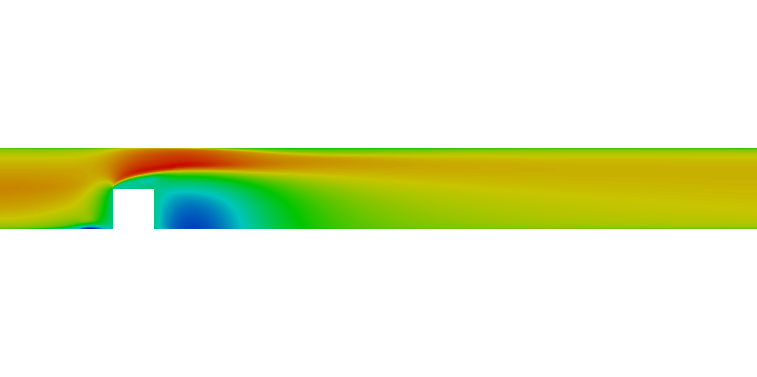
\includegraphics[scale=0.25]{figure/fine/eight/Umean_z.png}
\caption*{$f_k$=0.8}
\end{minipage}
\begin{minipage}[b]{0.5\linewidth}
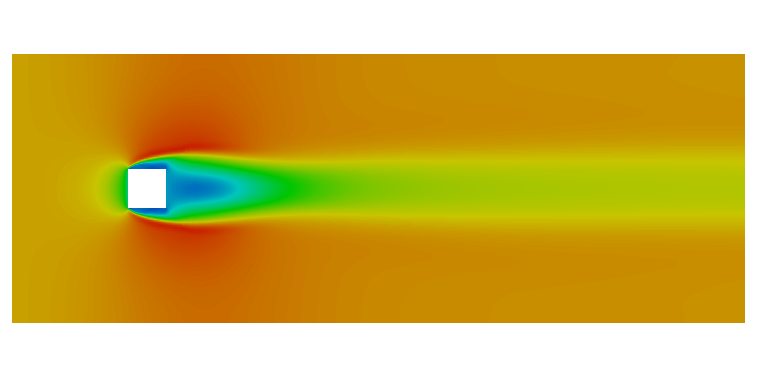
\includegraphics[scale=0.25]{figure/fine/eight/Umean_y.png}
\caption*{}
\end{minipage}\\
\begin{minipage}[b]{0.5\linewidth}
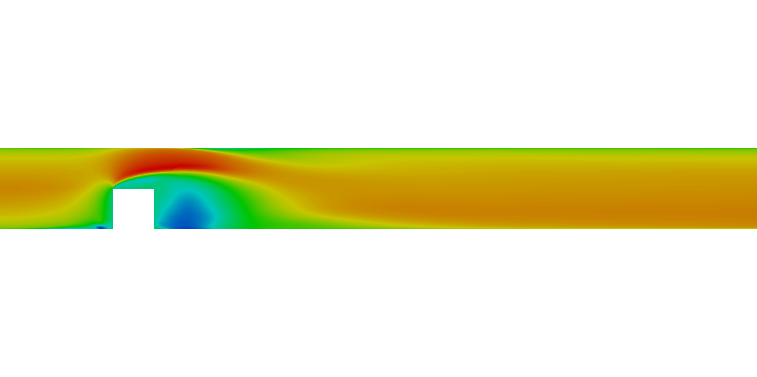
\includegraphics[scale=0.25]{figure/fine/three/Umean_z.png}
\caption*{$f_k$=0.3}
\end{minipage}
\begin{minipage}[b]{0.5\linewidth}
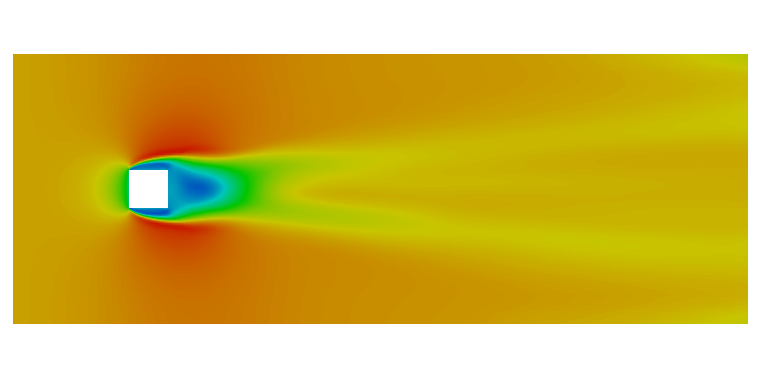
\includegraphics[scale=0.25]{figure/fine/three/Umean_y.png}
\caption*{}
\end{minipage}\\
\begin{minipage}[b]{0.5\linewidth}
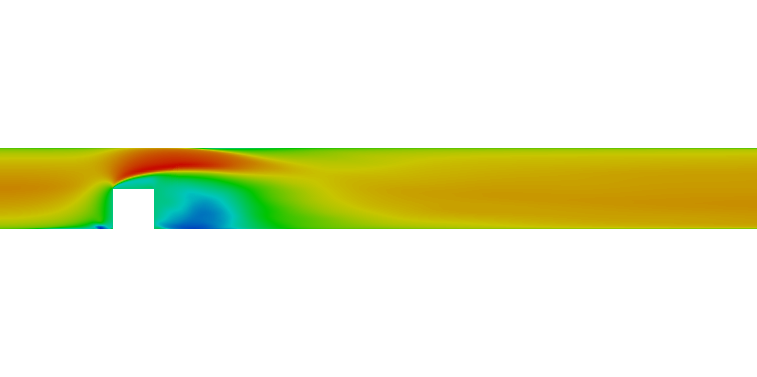
\includegraphics[scale=0.25]{figure/fine/one/Umean_z.png}
\caption*{$f_k$=0.15}
\end{minipage}
\begin{minipage}[b]{0.5\linewidth}
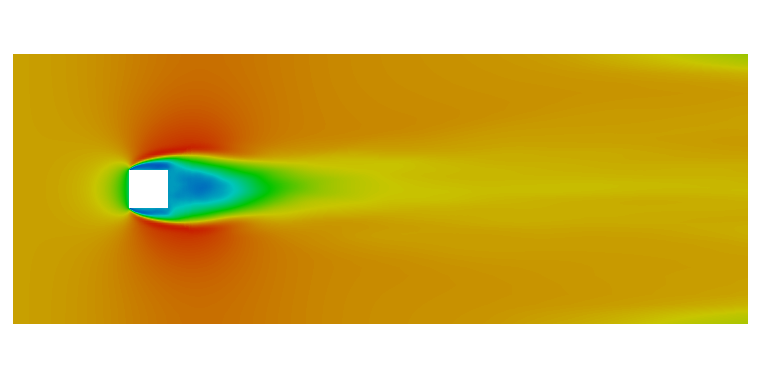
\includegraphics[scale=0.25]{figure/fine/one/Umean_y.png}
\caption*{}
\end{minipage}
\begin{minipage}[b]{0.5\linewidth}
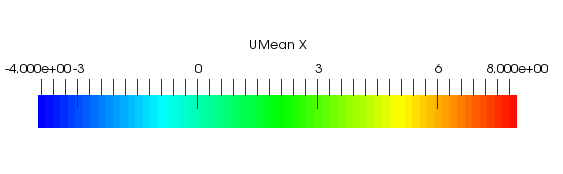
\includegraphics[scale=0.35]{figure/z_scale.png}
\end{minipage}
\begin{minipage}[b]{0.5\linewidth}
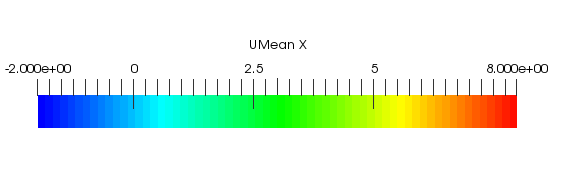
\includegraphics[scale=0.35]{figure/y_scale.png}
\end{minipage}\\

\caption{Mean velocity(U) plots about Z axis(left) and Y axis(right) for fine grid}
\label{fig:43}
\end{figure}


\section{Instantaneous Velocity Contour plots}



\begin{figure}[H]
\begin{minipage}[b]{0.5\linewidth}
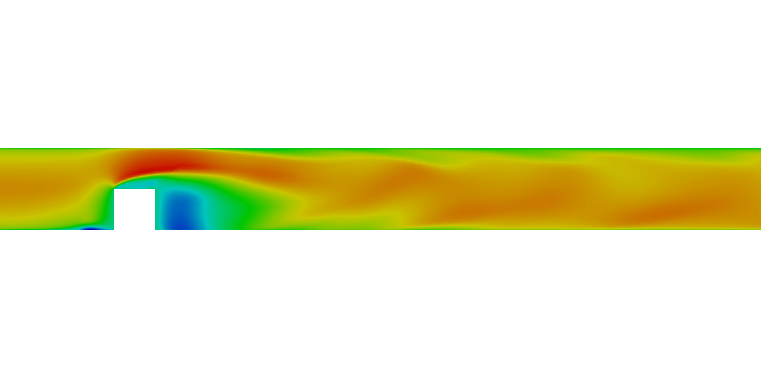
\includegraphics[scale=0.25]{figure/coarse/eight/Umag_z.png}
\caption*{$f_k$=0.8}
\end{minipage}
\begin{minipage}[b]{0.5\linewidth}
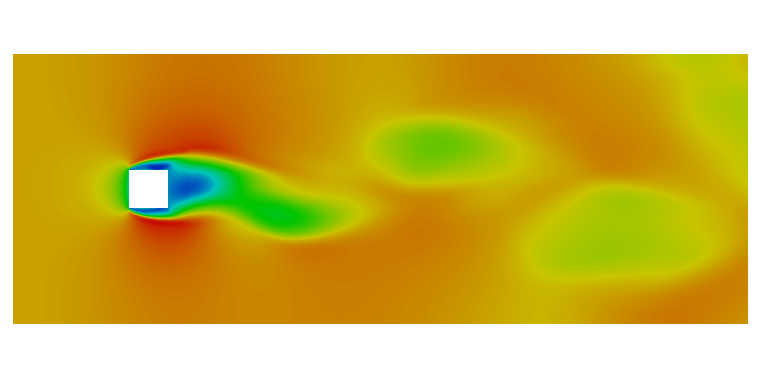
\includegraphics[scale=0.25]{figure/coarse/eight/Umag_y.png}
\caption*{}
\end{minipage}\\
\label{fig:eight}
\end{figure}
\newpage
\begin{figure}[H]
\ContinuedFloat
\begin{minipage}[b]{0.5\linewidth}
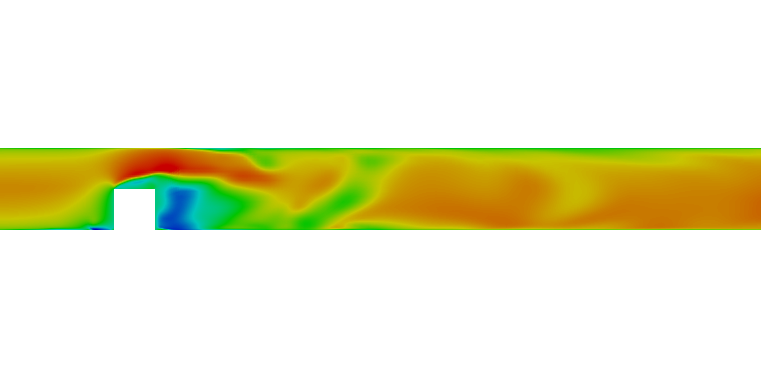
\includegraphics[scale=0.25]{figure/coarse/three/Umag_z.png}
\caption*{$f_k$=0.3}
\end{minipage}
\begin{minipage}[b]{0.5\linewidth}
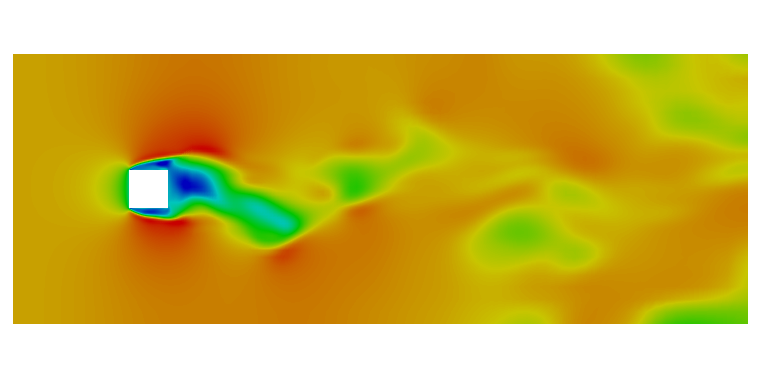
\includegraphics[scale=0.25]{figure/coarse/three/Umag_y.png}
\caption*{}
\end{minipage}\\

\begin{minipage}[b]{0.5\linewidth}
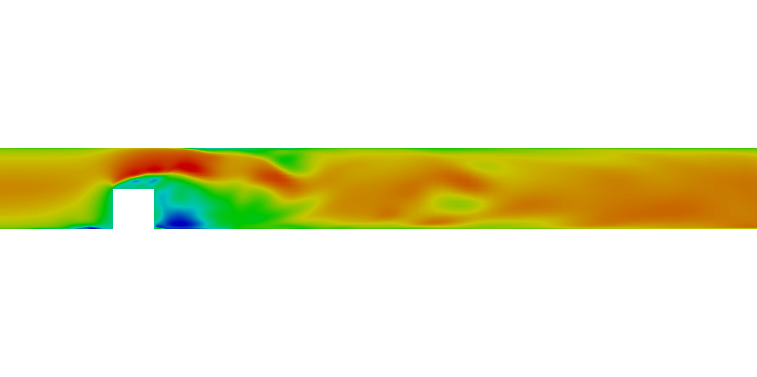
\includegraphics[scale=0.25]{figure/coarse/two/Umag_z.png}
\caption*{$f_k$=0.2}
\end{minipage}
\begin{minipage}[b]{0.5\linewidth}
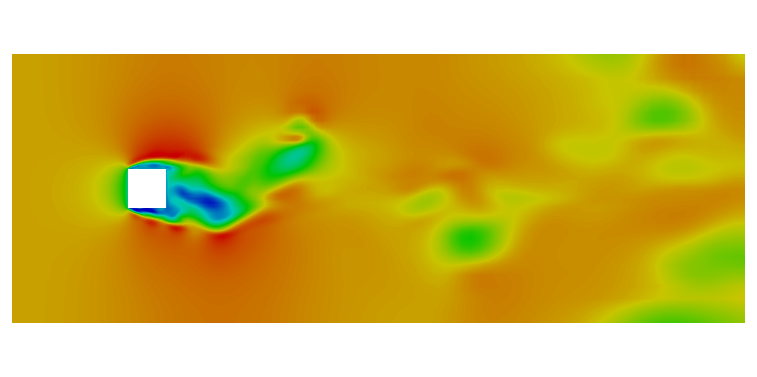
\includegraphics[scale=0.25]{figure/coarse/two/Umag_y.png}
\caption*{}
\end{minipage}
\begin{minipage}[b]{0.5\linewidth}
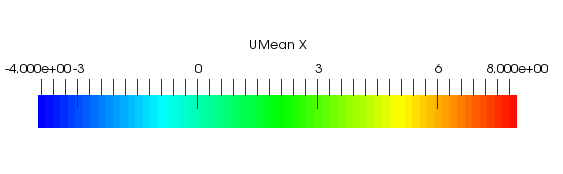
\includegraphics[scale=0.35]{figure/z_scale.png}
\end{minipage}
\begin{minipage}[b]{0.5\linewidth}
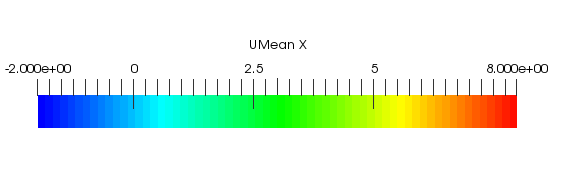
\includegraphics[scale=0.35]{figure/y_scale.png}
\end{minipage}\\
\caption{Instantaneous velocity(U) plots($t=4s$) about Z axis(left) and Y axis(right) for coarse grid}
\label{fig:43}
\end{figure}


Figures \ref{fig:43} and \ref{fig:44} give the instantaneous plots for U velocity at $t=4s$. The plots show the evolution of smaller flow structures with grid refinement and reducing $f_k$. 



\begin{figure}[H]
\begin{minipage}[b]{0.5\linewidth}
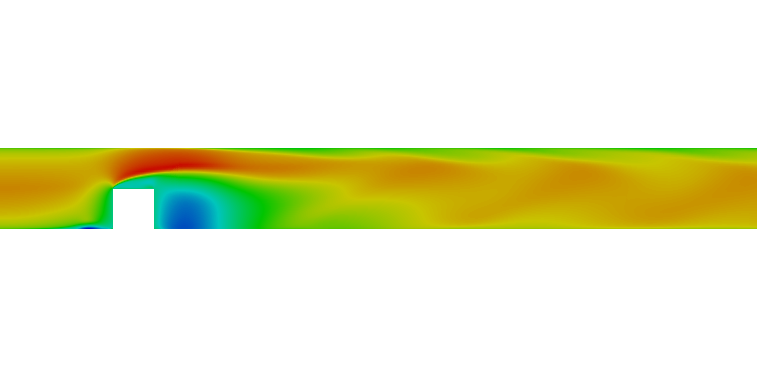
\includegraphics[scale=0.25]{figure/fine/eight/Umag_z.png}
\caption*{$f_k$=0.8}
\end{minipage}
\begin{minipage}[b]{0.5\linewidth}
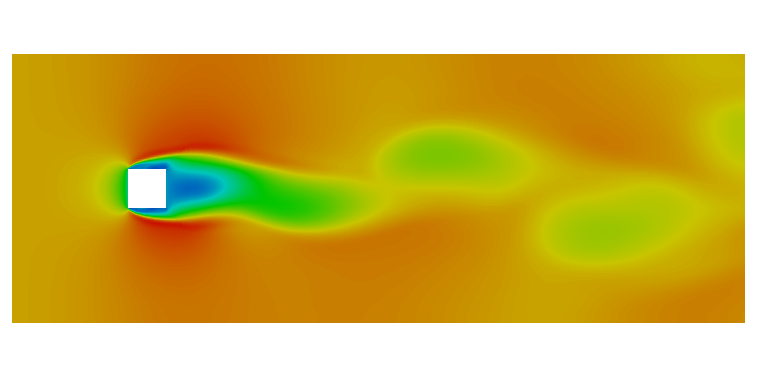
\includegraphics[scale=0.25]{figure/fine/eight/Umag_y.png}
\caption*{}
\end{minipage}\\
\caption{Instantaneous velocity(U) plots($t=4s$) about Z axis(left) and Y axis(right) for fine grid}
\label{fig:eight}
\end{figure}
\begin{figure}[H]
\ContinuedFloat
\begin{minipage}[b]{0.5\linewidth}
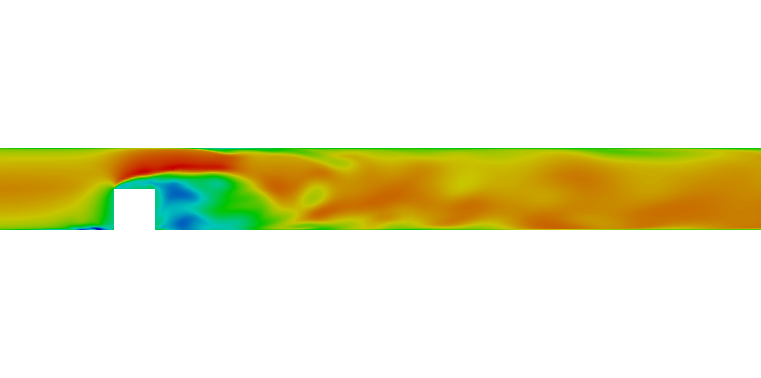
\includegraphics[scale=0.25]{figure/fine/three/Umag_z.png}
\caption*{$f_k$=0.3}
\end{minipage}
\begin{minipage}[b]{0.5\linewidth}
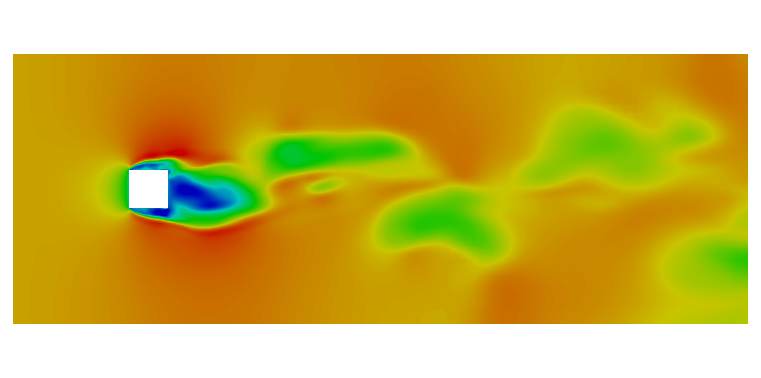
\includegraphics[scale=0.25]{figure/fine/three/Umag_y.png}
\caption*{}
\end{minipage}\\
\begin{minipage}[b]{0.5\linewidth}
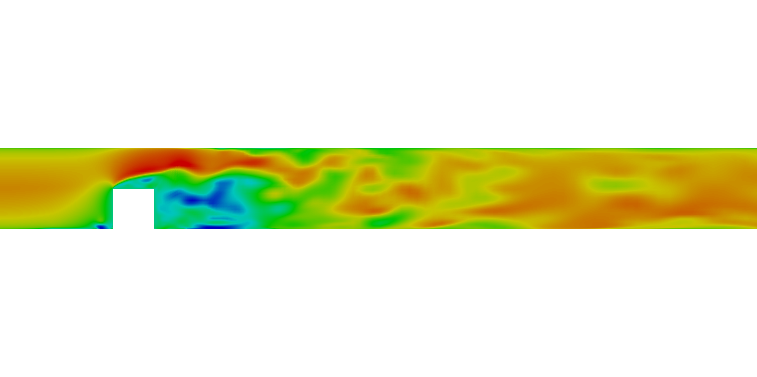
\includegraphics[scale=0.25]{figure/fine/one/Umag_z.png}
\caption*{$f_k$=0.15}
\end{minipage}
\begin{minipage}[b]{0.5\linewidth}
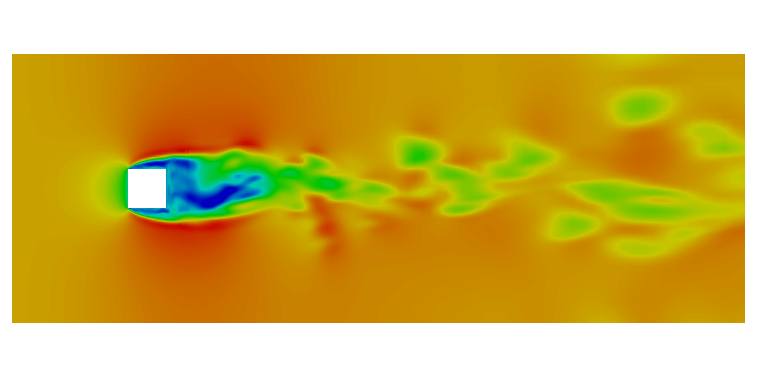
\includegraphics[scale=0.25]{figure/fine/one/Umag_y.png}
\caption*{}
\end{minipage}
\begin{minipage}[b]{0.5\linewidth}
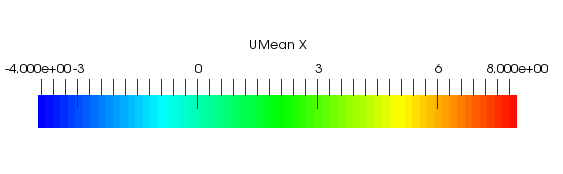
\includegraphics[scale=0.35]{figure/z_scale.png}
\end{minipage}
\begin{minipage}[b]{0.5\linewidth}
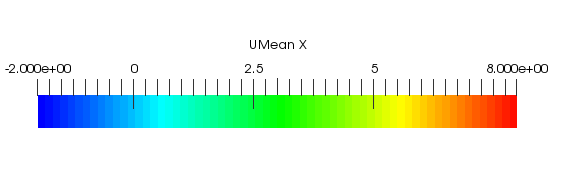
\includegraphics[scale=0.35]{figure/y_scale.png}
\end{minipage}\\
\caption{Instantaneous velocity(U) plots($t=4s$) about Z axis(left) and Y axis(right) for fine grid}
\label{fig:44}
\end{figure}



\section{Influence of $f_k$(input)}
Second invariant of velocity gradient $Q$, which is,  \(Q=-\frac{1}{2}(\frac{\partial u_i}{\partial x_j}\frac{\partial u_j}{\partial x_i})\) is an useful quantity in bluff body simulations to plot resolved flow structures. The term $u_i$ represents partially averaged velocity in PANS. The increasing capturing of smaller structures can be observed with the increase in both grid refinement and $f_k$(input).
\begin{figure}[H]
\begin{minipage}[b]{0.5\linewidth}
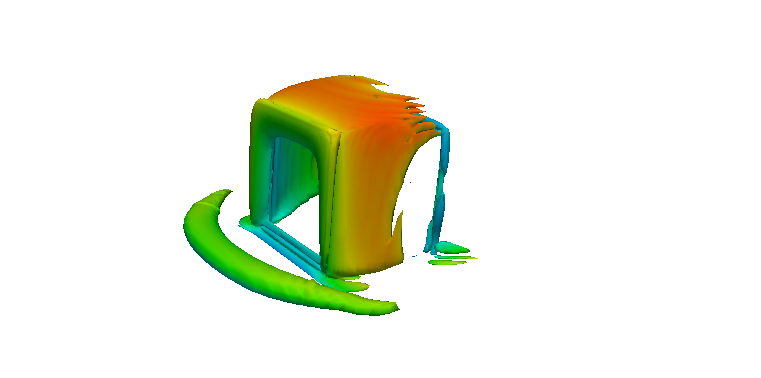
\includegraphics[scale=0.25]{figure/coarse/eight/iso.png}
\caption*{$f_k$=0.8}
\end{minipage}
\begin{minipage}[b]{0.5\linewidth}
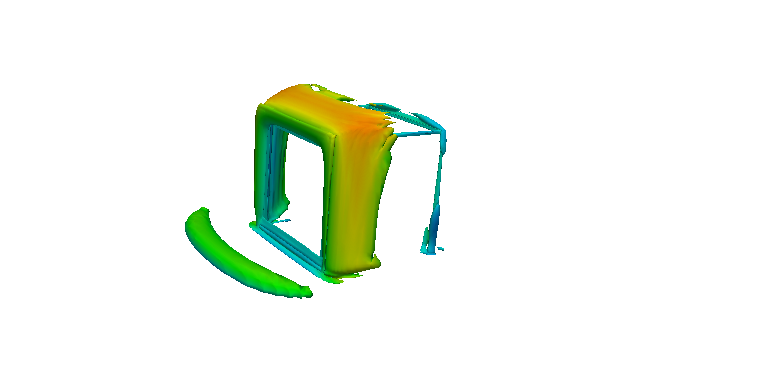
\includegraphics[scale=0.25]{figure/fine/eight/iso.png}
\caption*{$f_k$=0.8}
\end{minipage}\\
\caption{Iso-surface of Q-criterion coloured by Mean velocity(U) for coarse(left) and fine(right)}
\end{figure}
\begin{figure}[H]
\ContinuedFloat
\begin{minipage}[b]{0.5\linewidth}
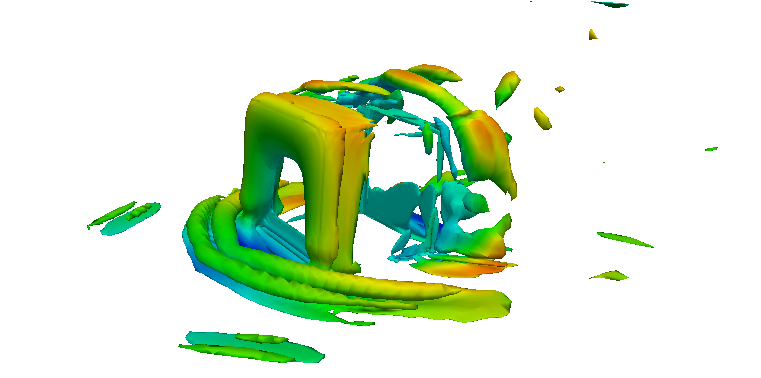
\includegraphics[scale=0.25]{figure/coarse/three/iso.png}
\caption*{$f_k$=0.3}
\end{minipage}
\begin{minipage}[b]{0.5\linewidth}
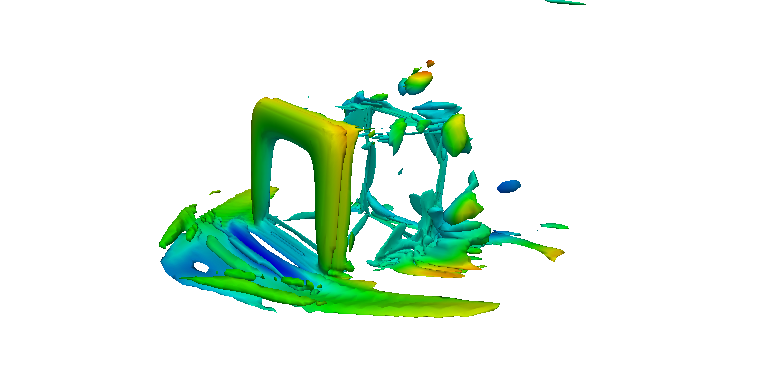
\includegraphics[scale=0.25]{figure/fine/three/iso.png}
\caption*{$f_k$=0.3}
\end{minipage}\\
\begin{minipage}[b]{0.5\linewidth}
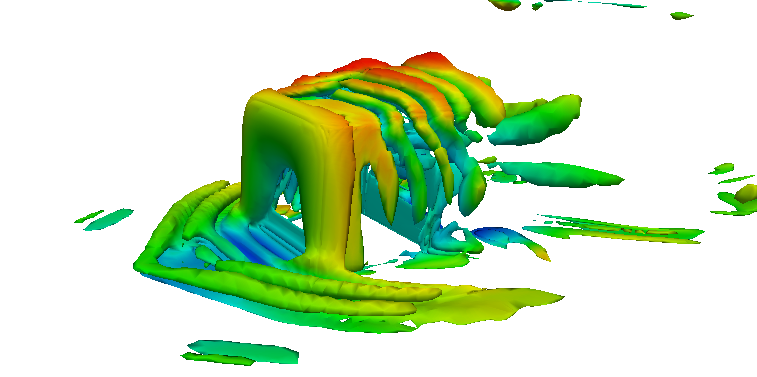
\includegraphics[scale=0.25]{figure/coarse/two/iso.png}
\caption*{$f_k$=0.2}
\end{minipage}
\begin{minipage}[b]{0.5\linewidth}
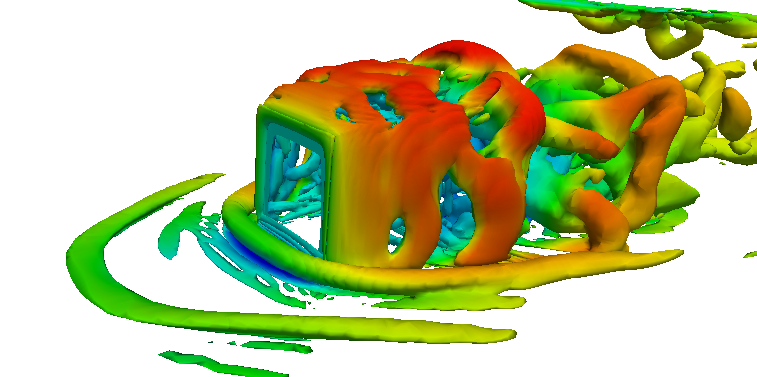
\includegraphics[scale=0.25]{figure/fine/one/iso.png}
\caption*{$f_k$=0.15}
\end{minipage}
\begin{center}
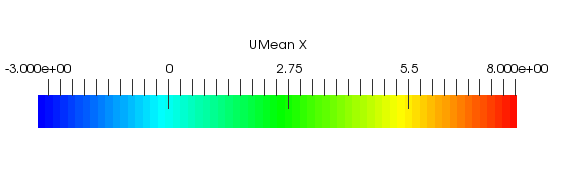
\includegraphics[scale=0.5]{figure/iso_scale.png}
\end{center}
\caption{Iso-surface of Q-criterion coloured by Mean velocity(U) for coarse(left) and fine(right)}
\end{figure}


\begin{comment}
\begin{figure}[H]
\begin{minipage}[b]{0.5\linewidth}
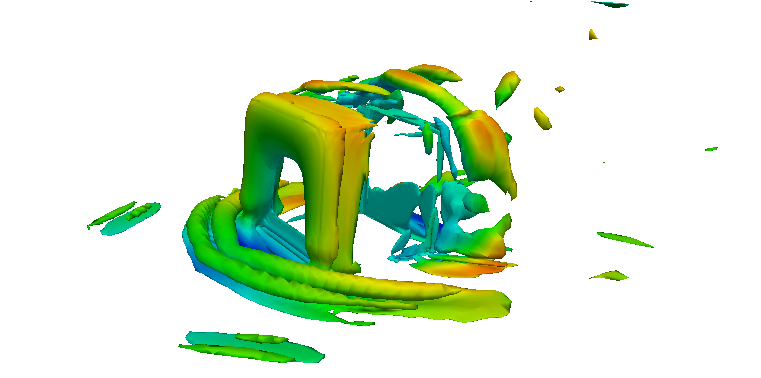
\includegraphics[scale=0.25]{figure/coarse/three/iso.png}
\end{minipage}
\begin{minipage}[b]{0.5\linewidth}
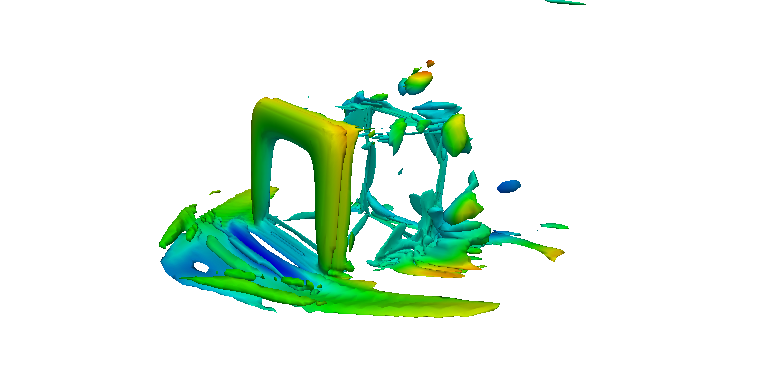
\includegraphics[scale=0.25]{figure/fine/three/iso.png}
\end{minipage}
\caption{Iso-surface of Q-criterion coloured by Mean velocity(U) for coarse(left, $f_k$=0.3) and fine(right, $f_k$=0.3)}
\end{figure}

\begin{figure}[H]
\begin{minipage}[b]{0.5\linewidth}
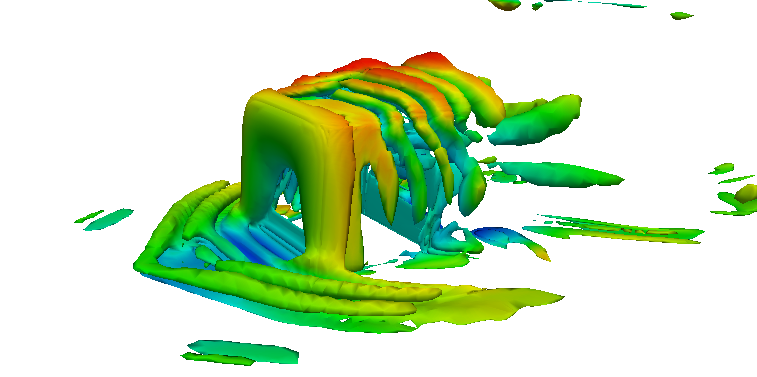
\includegraphics[scale=0.25]{figure/coarse/two/iso.png}
\end{minipage}
\begin{center}
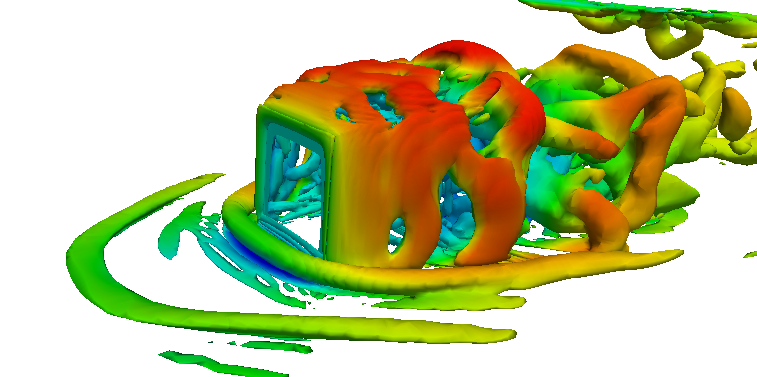
\includegraphics[scale=0.25]{figure/fine/one/iso.png}
\end{center}
\caption{Iso-surface of Q-criterion coloured by Mean velocity(U) for coarse(left, $f_k$=0.2) and fine(right, $f_k$=0.15)}
\end{figure}
\end{comment}

\section{$f_k$(output) plots}
\hspace{0.25cm}Figures \ref{fig:46} and \ref{fig:47} represent the influence of grid refinement and changing $f_k$(input) on $f_k$(output). It can be observed that the structures are more resolved with increasing grid refinement. 

\begin{figure}[H]
\begin{minipage}[b]{0.5\linewidth}
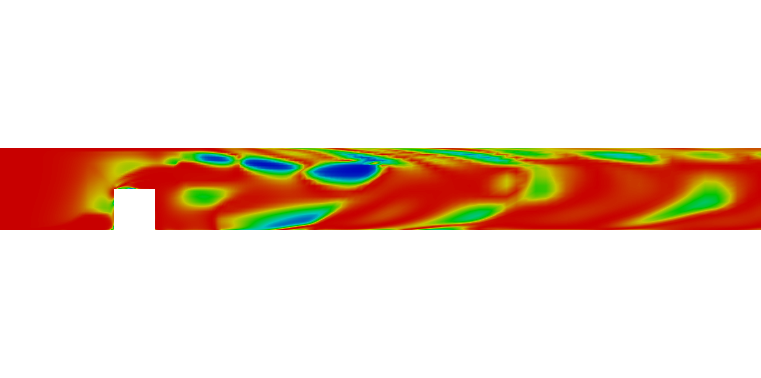
\includegraphics[scale=0.25]{figure/coarse/eight/fkout_z.png}
\caption*{$f_k$=0.8}
\end{minipage}
\begin{minipage}[b]{0.5\linewidth}
\includegraphics[scale=0.25]{figure/coarse/eight/fkout_y.png}
\caption*{}
\end{minipage}\\
\caption{$f_k$(output) plots about Z axis(left) and Y axis(right) for coarse grid}
\label{fig:eight}
\end{figure}

\begin{figure}[H]
\ContinuedFloat
\begin{minipage}[b]{0.5\linewidth}
\includegraphics[scale=0.25]{figure/coarse/three/fkout_z.png}
\caption*{$f_k$=0.3}
\end{minipage}
\begin{minipage}[b]{0.5\linewidth}
\includegraphics[scale=0.25]{figure/coarse/three/fkout_y.png}
\caption*{}
\end{minipage}\\
\begin{minipage}[b]{0.5\linewidth}
\includegraphics[scale=0.25]{figure/coarse/two/fkout_z.png}
\caption*{$f_k$=0.2}
\end{minipage}
\begin{minipage}[b]{0.5\linewidth}
\includegraphics[scale=0.25]{figure/coarse/two/fkout_y.png}
\caption*{}
\end{minipage}
\begin{center}
\includegraphics[scale=0.5]{figure/fk_scale.png}
\end{center}
\caption{$f_k$(output) plots about Z axis(left) and Y axis(right) for coarse grid}
\label{fig:46}
\end{figure}
On the higher spectrum of $f_k$, the results tend to be very dissipative. This could be because of the k-$\omega$ turbulence model is generally dissipative. But it seems to follow the flow pattern and resolve in important regions in the flow. Also, it can be observed through $f_k$(ouput) plots that more structures are released with increasing grid refinement and $f_k$(input).




 
\begin{figure}[H]
\begin{minipage}[b]{0.5\linewidth}
\includegraphics[scale=0.25]{figure/fine/eight/fkout_z.png}
\caption*{$f_k$=0.8}
\end{minipage}
\begin{minipage}[b]{0.5\linewidth}
\includegraphics[scale=0.25]{figure/fine/eight/fkout_y.png}
\caption*{}
\end{minipage}\\
\caption{$f_k$(output) plots about Z axis(left) and Y axis(right) for fine grid}
\label{fig:eight}
\end{figure}
\begin{figure}[H]
\ContinuedFloat
\begin{minipage}[b]{0.5\linewidth}
\includegraphics[scale=0.25]{figure/fine/three/fkout_z.png}
\caption*{$f_k$=0.3}
\end{minipage}
\begin{minipage}[b]{0.5\linewidth}
\includegraphics[scale=0.25]{figure/fine/three/fkout_y.png}
\caption*{}
\end{minipage}\\
\begin{minipage}[b]{0.5\linewidth}
\includegraphics[scale=0.25]{figure/fine/one/fkout_z.png}
\caption*{$f_k$=0.15}
\end{minipage}
\begin{minipage}[b]{0.5\linewidth}
\includegraphics[scale=0.25]{figure/fine/one/fkout_y.png}
\caption*{}
\end{minipage}
\begin{center}
 \includegraphics[scale=0.5]{figure/fk_scale.png}
\end{center}
\caption{$f_k$(output) plots about Z axis(left) and Y axis(right) for fine grid}
\label{fig:47}
\end{figure}



\section{Line plots}
A study of different line plots at locations, \(\frac{x}{H}=0.5\) and \(\frac{x}{H}=2\). The obtained results are compared with the experimental results. 

\begin{figure}[H]
\begin{minipage}[b]{0.5\linewidth}
\includegraphics[scale=0.5]{figure/coarse/U_coarse_five.pdf}
\end{minipage}
\begin{minipage}[b]{0.5\linewidth}
\includegraphics[scale=0.5]{figure/fine/U_fine_five.pdf}
\end{minipage}\\
\caption{Mean velocity(U) profile for coarse(left) and fine(right) grids}
\label{fig:eight}
\end{figure}
\begin{figure}[H]
\ContinuedFloat
\begin{minipage}[b]{0.5\linewidth}
\includegraphics[scale=0.5]{figure/coarse/U_coarse_two.pdf}
\end{minipage}
\begin{minipage}[b]{0.5\linewidth}
\includegraphics[scale=0.5]{figure/fine/U_fine_two.pdf}
\end{minipage}
\caption{Mean velocity(U) profile for coarse(left) and fine(right) grids}
\label{fig:48}
\end{figure}

\begin{comment}
\begin{figure}[H]
\begin{minipage}[b]{0.5\linewidth}
\includegraphics[scale=0.5]{figure/coarse/U_coarse_two.pdf}
\end{minipage}
\begin{minipage}[b]{0.5\linewidth}
\includegraphics[scale=0.5]{figure/fine/U_fine_two.pdf}
\end{minipage}
\caption{Mean velocity(U) profile for coarse(left) and fine(right) grids}
\label{fig:eight}
\end{figure}

\end{comment}
Both the U and V plots seem to be in close agreement with the experimental results apart from the V plot for the fine grid at \(\frac{x}{H}=2\) in figure \ref{fig:49}. It can also be observed in figure \ref{fig:48} for coarse grid at \(\frac{x}{H}=0.5\), $f_k$(input) of 0.8 performs better than others. The reason for this could be usage of a higher value of $f_k$(input) seems unnecessary for the coarse grid.

\begin{figure}[H]
\begin{minipage}[b]{0.5\linewidth}
\includegraphics[scale=0.5]{figure/coarse/V_coarse_five.pdf}
\end{minipage}
\begin{minipage}[b]{0.5\linewidth}
\includegraphics[scale=0.5]{figure/fine/V_fine_five.pdf}
\end{minipage}\\
\begin{minipage}[b]{0.5\linewidth}
\includegraphics[scale=0.5]{figure/coarse/V_coarse_two.pdf}
\end{minipage}
\begin{minipage}[b]{0.5\linewidth}
\includegraphics[scale=0.5]{figure/fine/V_fine_two.pdf}
\end{minipage}
\caption{Mean velocity(V) profile for coarse(left) and fine(right) grids}
\label{fig:49}
\end{figure}


\begin{comment}
\begin{figure}[H]
\begin{minipage}[b]{0.5\linewidth}
\includegraphics[scale=0.5]{figure/coarse/V_coarse_two.pdf}
\end{minipage}
\begin{minipage}[b]{0.5\linewidth}
\includegraphics[scale=0.5]{figure/fine/V_fine_two.pdf}
\end{minipage}
\caption{Mean velocity(V) profile for coarse(left) and fine(right) grids}
\label{fig:eight}
\end{figure}
\end{comment}




\begin{figure}[H]
\begin{minipage}[b]{0.5\linewidth}
\includegraphics[scale=0.5]{figure/coarse/UU_coarse_five.pdf}
\end{minipage}
\begin{minipage}[b]{0.5\linewidth}
\includegraphics[scale=0.5]{figure/fine/UU_fine_five.pdf}
\end{minipage}\\
\begin{minipage}[b]{0.5\linewidth}
\includegraphics[scale=0.5]{figure/coarse/UU_coarse_two.pdf}
\end{minipage}
\begin{minipage}[b]{0.5\linewidth}
\includegraphics[scale=0.5]{figure/fine/UU_fine_two.pdf}
\end{minipage}
\caption{Normalized stress($<u^{'}u^{'}>$) profile for coarse(left) and fine(right) grids}
\label{fig:eight}
\end{figure}
Figures above represent the normalized resolved stresses at the above mentioned locations. It can be observed that with the increasing $f_k$(input) value more fluctuations is observed at the locations.

\begin{comment}
\begin{figure}[H]
\begin{minipage}[b]{0.5\linewidth}
\includegraphics[scale=0.5]{figure/coarse/UU_coarse_two.pdf}
\end{minipage}
\begin{minipage}[b]{0.5\linewidth}
\includegraphics[scale=0.5]{figure/fine/UU_fine_two.pdf}
\end{minipage}
\caption{Normalized stress($<u^{'}u^{'}>$) profile for coarse(left) and fine(right) grids}
\label{fig:eight}
\end{figure}

\end{comment}

\section{Conclusions}
PANS was implemented for k-$\omega$ turbulence model in OpenFOAM. PANS seems to capture the flow structures satisfactorily. PANS seamlessly varies between RANS and DNS as the results show. The obtained results were validated with experimental results and they seem to agree closely. 


\section{Future work}
The work shows that PANS can provide intermediate accuracy at intermediate costs. A more optimized method to obtain $f_k$(input) is required in order to efficiently solve industrial problems. In real time applications there are always time varying boundary conditions. Intuitively, it can be seen that there is a requirement of a dynamic $f_k$(input) required to accommodate for these changes. In order to achieve this, the governing equations of the closure models need to be changed to adapt to the changing $f_k$(input). Some of the line plots are not in good agreement with the experimental results. This could be due to numerical errors since the case was not tested with varying numerical schemes. Therefore, a study to investigate this could be performed in the future. 






































% CONCLUSION

% REFERENCES / BIBLIOGRAPHY
\cleardoublepage
\addcontentsline{toc}{chapter}{Bibliography}
% CREATED BY DAVID FRISK, 2015
\begin{thebibliography}{69}




\bibitem{petsc} PETSc Users Manual(Revision 3.7), Mathematics and Computer Science Division, Argonne National Laboratory.




\end{thebibliography}


% APPENDICES
\cleardoublepage
%\appendix
\setcounter{secnumdepth}{0}
%\appendix
\chapter{Preferred Direction Diffusion Scheme}
This chapter provides a detailed derivation of the integral calculations to obtain the coefficients in (\ref{eq:a21}).
\label{app:aa}
\section{Cell Properties}
\label{sec:one}
\begin{comment}
\begin{figure}[H]
\centering
\includegraphics[scale=0.6]{include/backmatter/cdd.JPG}
\caption{Representation of a cell in Physical Space}
\label{fig:cellp}
\end{figure}
\end{comment}
Twenty cell properties are calculated for each cell using an uniquely defined reference node point $(x_{ref},y_{ref},z_{ref})$ .
\begin{equation}\label{eq:eqns}
\begin{gathered}
\nonumber
\mathcal{V}_{o_k}=\int\int\int_{\Omega_k}d\Omega \\
\mathcal{V}_{x_k}=\int\int\int_{\Omega_k}(x-x_{ref})d\Omega\\ 
\mathcal{V}_{y_k}=\int\int\int_{\Omega_k}(y-y_{ref})d\Omega\\ 
\mathcal{V}_{z_k}=\int\int\int_{\Omega_k}(z-z_{ref})d\Omega\\ 
\mathcal{V}_{xx_k}=\int\int\int_{\Omega_k}(x-x_{ref})^2d\Omega\\ 
\mathcal{V}_{xy_k}=\int\int\int_{\Omega_k}(x-x_{ref})(y-y_{ref})d\Omega\\ 
\mathcal{V}_{xz_k}=\int\int\int_{\Omega_k}(x-x_{ref})(z-z_{ref})d\Omega\\ 
\mathcal{V}_{yy_k}=\int\int\int_{\Omega_k}(y-y_{ref})^2d\Omega\\ 
\mathcal{V}_{yz_k}=\int\int\int_{\Omega_k}(y-y_{ref})(z-z_{ref})d\Omega\\ 
\mathcal{V}_{zz_k}=\int\int\int_{\Omega_k}(z-z_{ref})^2d\Omega\\ 
\mathcal{V}_{xxx_k}=\int\int\int_{\Omega_k}(x-x_{ref})^3d\Omega\\ 
\mathcal{V}_{xxy_k}=\int\int\int_{\Omega_k}(x-x_{ref})^2(y-y_{ref})d\Omega\\ 
\mathcal{V}_{xxz_k}=\int\int\int_{\Omega_k}(x-x_{ref})^2(z-z_{ref})d\Omega\\ 
\mathcal{V}_{xyy_k}=\int\int\int_{\Omega_k}(x-x_{ref})(y-y_{ref})^2d\Omega\\ 
\frac{\partial (\rho k)}{\partial t}+\frac{\partial (\rho k <V_j>)}{\partial x_j}=P_k-\beta^*k w+\frac{\partial}{\partial x_j}(\Gamma_{k}\frac{\partial k}{\partial x_j})\\
\frac{\partial (\rho \omega)}{\partial t}+\frac{\partial (\rho \omega <V_j>)}{\partial x_j}=\frac{\gamma}{\nu}P_k-\beta\rho\omega^2+\frac{\partial}{\partial x_j}(\Gamma_{\omega}\frac{\partial \omega}{\partial x_j})+2(1-F_1)\sigma_{w2}\frac{1}{\omega}\frac{\partial k}{\partial x_j}\frac{\partial \omega}{\partial x_j}
\end{gathered}
\end{equation}\\
\begin{equation}\label{fig:other}
\begin{gathered}
\mathcal{V}_{xyz_k}=\int\int\int_{\Omega_k}(x-x_{ref})(y-y_{ref})(z-z_{ref})d\Omega\\ 
\mathcal{V}_{xzz_k}=\int\int\int_{\Omega_k}(x-x_{ref})(z-z_{ref})^2d\Omega\\ 
\mathcal{V}_{yyy_k}=\int\int\int_{\Omega_k}(y-y_{ref})^3d\Omega\\ 
\mathcal{V}_{yyz_k}=\int\int\int_{\Omega_k}(y-y_{ref})^2(z-z_{ref})d\Omega\\ 
\mathcal{V}_{yzz_k}=\int\int\int_{\Omega_k}(y-y_{ref})(z-z_{ref})^2d\Omega\\ 
\mathcal{V}_{zzz_k}=\int\int\int_{\Omega_k}(z-z_{ref})^3d\Omega\\
\frac{\partial (\rho k)}{\partial t}+\frac{\partial (\rho k <V_j>)}{\partial x_j}=P_k-\beta^*k w+\frac{\partial}{\partial x_j}(\Gamma_{k}\frac{\partial k}{\partial x_j})
\frac{\partial (\rho \omega)}{\partial t}+\frac{\partial (\rho \omega <V_j>)}{\partial x_j}=\frac{\gamma}{\nu}P_k-\beta\rho\omega^2+\frac{\partial}{\partial x_j}(\Gamma_{\omega}\frac{\partial \omega}{\partial x_j})+2(1-F_1)\sigma_{w2}\frac{1}{\omega}\frac{\partial k}{\partial x_j}\frac{\partial \omega}{\partial x_j}
 \end{gathered}
\end{equation}
\section*{Tri-Linear Parametrization}
The Cell properties in \ref{sec:one} are calculated for each of the ten cells per face using Gauss-point Quadrature. Initially a local coordinate system $(x',y',z')$ is defined for each cell. This system with respect to the global co-ordinate system is obtained using tri-linear parametrization. 
\begin{figure}[h]
\centering
\includegraphics[height=8cm]{include/backmatter/tlp.JPG}
\caption{Representation of local co-ordinate sytem of a cell in physical space }
\label{fig:tlpcell}
\end{figure}
\begin{equation}\label{eq:tlm}
 \begin{gathered}
 x=(1-x')(1-y')(1-z')x_0+x'(1-y')(1-z')x_1+\\
 (1-x')y'(1-z')x_2+x'y'(1-z')x_3+(1-x')(1-y')z'x_4+\\
 x'(1-y')z'x_5+(1-x')y'z'x_6+x'y'z'x_7 \\
 y=(1-x')(1-y')(1-z')y_0+x'(1-y')(1-z')y_1+\\
 (1-x')y'(1-z')y_2+x'y'(1-z')y_3+(1-x')(1-y')z'y_4+\\
 x'(1-y')z'y_5+(1-x')y'z'y_6+x'y'z'y_7 \\
 z=(1-x')(1-y')(1-z')z_0+x'(1-y')(1-z')z_1+\\
 (1-x')y'(1-z')z_2+x'y'(1-z')z_3+(1-x')(1-y')z'z_4+\\
 x'(1-y')z'z_5+(1-x')y'z'z_6+x'y'z'z_7 \\
 \end{gathered}
 \end{equation}
 \section*{Gauss-point Quadrature}\label{sec:gpq}
 Using the equations in (\ref{eq:tlm}), the volume integrals in (\ref{eq:eqns}) are calculated using Gauss-point Quadrature numerical integration method. The general representation of the integration is given by,
 \begin{equation}
 \begin{gathered}
     \label{eq:gauss}
     \int\int\int_{\Omega_k} \phi(x,y,z) \,dxdydz=\int_{0}^{1}\int_{0}^{1}\int_{0}^{1}\phi(x',y',z')J\,dx'dy'dz'\\
     $where Jacobian J is defined as,$\\
     \begin{vmatrix}
    \frac{\partial x}{\partial x'} & \frac{\partial x}{\partial y'} & \frac{\partial x}{\partial z'}\\
    \frac{\partial y}{\partial x'} & \frac{\partial y}{\partial y'} & \frac{\partial y}{\partial z'}\\
    \frac{\partial z}{\partial x'} & \frac{\partial z}{\partial y'} & \frac{\partial z}{\partial z'}
    \end{vmatrix}
     \end{gathered}
 \end{equation}
 In order to use the Gauss-point quadrature, the range of the local coordinate system must be redefined from -1 to 1.
 \begin{equation}
 \begin{gathered}
     \label{eq:gaussfinal}
     \int\int\int_{\Omega_k} \phi(x,y,z)\,dxdydz=\frac{1}{8}\int_{-1}^{1}\int_{-1}^{1}\int_{-1}^{1}\phi(x'',y'',z'')J(x'',y'',z'')\,dx''dy''dz''
     \end{gathered}
     \end{equation}
     \begin{equation}
     \label{eq:gaussfinal2}
     \int\int\int_{\Omega_k} \phi(x,y,z)\,dxdydz=\frac{1}{8}\sum\limits_{i=1}^{n}\sum\limits_{j=1}^{n}\sum\limits_{k=1}^{n}w_iw_jw_k\phi(p_i,p_j,p_k)J(p_i,p_j,p_k)
     \end{equation}
     Where $p_i,p_j,p_k$ are the Gauss points and $w_i,w_j,w_k$ are the corresponding weights.
     
    
\section*{Volume Integrals}\label{sec:vi}
The integrals in matrix $A$ is calculated using the relationship between the $(\xi,\eta,\zeta)$ space and $(x,y,z)$ space in (\ref{eq:lcs}).
\begin{equation}
    \label{eq:a11}
    \begin{gathered}
    \xi=\Psi_{11}(x-x_o)+\Psi_{12}(y-y_o)+\Psi_{13}(z-z_o)\\
    \eta=\Psi_{21}(x-x_o)+\Psi_{22}(y-y_o)+\Psi_{23}(z-z_o)\\
    \zeta=\Psi_{31}(x-x_o)+\Psi_{32}(y-y_o)+\Psi_{33}(z-z_o)\\
    \end{gathered}
\end{equation}
The following relations are used to rewrite the integrals,
\begin{equation}
    \label{eq:a12}
    \begin{gathered}
    (x-x_o)=((x-x_{ref})+(x_{ref}-x_o))\\
    (y-y_o)=((y-y_{ref})+(y_{ref}-y_o))\\
    (z-z_o)=((z-z_{ref})+(z_{ref}-z_o))\\
    \end{gathered}
\end{equation}
Introducing the constansts $\Delta x,\Delta y,\Delta z$,
\begin{equation}
    \label{eq:a13}
    \begin{gathered}
    \Delta x=x_{ref}-x_o\\
    \Delta y=y_{ref}-y_o\\
    \Delta z=z_{ref}-z_o\\
    \end{gathered}
\end{equation}
which results in,
\begin{equation}
    \label{eq:a14}
    \begin{gathered}
    (x-x_o)=((x-x_{ref})+\Delta x)\\
    (y-y_o)=((y-y_{ref})+\Delta y)\\
    (z-z_o)=((z-z_{ref})+\Delta z)\\
    \end{gathered}
\end{equation}
The terms in the first column are obtained using the volume integrals in equations (\ref{eq:eqns}). Further, the second, third and fourth columns which consists of first order terms are obtained using the direct relations from equations (\ref{eq:a11}-\ref{eq:a14}).
\begin{equation}
    \label{eq:a15}
    \begin{gathered}
    \int\int\int_{\Omega_k}\xi\,d\Omega=\Psi_{11}(\mathcal{V}_{x_k}+\Delta x\mathcal{V}_{o_k})+\Psi_{12}(\mathcal{V}_{y_k}+\Delta y\mathcal{V}_{o_k})+\Psi_{13}(\mathcal{V}_{z_k}+\Delta z\mathcal{V}_{o_k})\\
    \int\int\int_{\Omega_k}\eta\,d\Omega=\Psi_{21}(\mathcal{V}_{x_k}+\Delta x\mathcal{V}_{o_k})+\Psi_{22}(\mathcal{V}_{y_k}+\Delta y\mathcal{V}_{o_k})+\Psi_{23}(\mathcal{V}_{z_k}+\Delta z\mathcal{V}_{o_k})\\
    \int\int\int_{\Omega_k}\zeta\,d\Omega=\Psi_{31}(\mathcal{V}_{x_k}+\Delta x\mathcal{V}_{o_k})+\Psi_{32}(\mathcal{V}_{y_k}+\Delta y\mathcal{V}_{o_k})+\Psi_{33}(\mathcal{V}_{z_k}+\Delta z\mathcal{V}_{o_k})\\
    \end{gathered}
\end{equation}
Further, the quadratic and cubic terms in matrix $A$ are calculated by rewriting and expanding the products of $\xi$, $\eta$ and $\zeta$.
\begin{equation}
    \label{eq:a16}
    \begin{gathered}
    \xi\eta=\Psi_{11}\Psi_{21}(x-x_o)^2+(\Psi_{11}\Psi_{22}+\Psi_{12}\Psi_{21})(x-x_o)(y-y_o)+\\
    (\Psi_{11}\Psi_{23}+\Psi_{13}\Psi_{21})(x-x_o)(z-z_o)+\Psi_{12}\Psi_{22}(y-y_o)^2+\\
    (\Psi_{12}\Psi_{23}+\Psi_{13}\Psi_{22}(y-y_o)(z-z_o)+\Psi_{13}\Psi_{23}(z-z_o)^2\\
    \xi\zeta=\Psi_{11}\Psi_{31}(x-x_o)^2+(\Psi_{11}\Psi_{32}+\Psi_{12}\Psi_{31})(x-x_o)(y-y_o)+\\
    (\Psi_{11}\Psi_{33}+\Psi_{13}\Psi_{31})(x-x_o)(z-z_o)+\Psi_{12}\Psi_{32}(y-y_o)^2+\\
    (\Psi_{12}\Psi_{33}+\Psi_{13}\Psi_{32}(y-y_o)(z-z_o)+\Psi_{13}\Psi_{33}(z-z_o)^2\\
    \\
    \zeta^2=\Psi_{21}\Psi_{21}(x-x_o)^2+2\Psi_{21}\Psi_{22}(x-x_o)(y-y_o)+\\
    2\Psi_{21}\Psi_{23}(x-x_o)(z-z_o)+\Psi_{22}\Psi_{22}(y-y_o)^2+\\
    2\Psi_{22}\Psi_{23}(y-y_o)(z-z_o)+\Psi_{23}\Psi_{23}(z-z_o)^2\\
    \eta^2=\Psi_{31}\Psi_{31}(x-x_o)^2+2\Psi_{31}\Psi_{32}(x-x_o)(y-y_o)+\\
    2\Psi_{31}\Psi_{33}(x-x_o)(z-z_o)+\Psi_{32}\Psi_{32}(y-y_o)^2+\\
    2\Psi_{32}\Psi_{33}(y-y_o)(z-z_o)+\Psi_{33}\Psi_{33}(z-z_o)^2\\
    \\
    \xi\eta^2=\Psi_{11}\Psi_{21}\Psi_{21}(x-x_o)^3+\\
    (2\Psi_{11}\Psi_{21}\Psi_{22}+\Psi_{12}\Psi_{21}\Psi_{21})(x-x_o)^2(y-y_o)+\\
    (2\Psi_{11}\Psi_{21}\Psi_{23}+\Psi_{13}\Psi_{21}\Psi_{21})(x-x_o)^2(z-z_o)+\\
    (\Psi_{11}\Psi_{22}\Psi_{22}+2\Psi_{12}\Psi_{21}\Psi_{22})(x-x_o)(y-y_o)^2+\\
    (2\Psi_{11}\Psi_{22}\Psi_{23}+2\Psi_{12}\Psi_{21}\Psi_{23}+2\Psi_{13}\Psi_{21}\Psi_{22})\\
    (x-x_o)(y-y_o)(z-z_o)+\\
    (\Psi_{11}\Psi_{23}\Psi_{23}+2\Psi_{13}\Psi_{21}\Psi_{23})(x-x_o)(z-z_o)^2+\\
    \Psi_{12}\Psi_{22}\Psi_{22}(y-y_o)^3+\\
    (2\Psi_{12}\Psi_{22}\Psi_{23}+\Psi_{13}\Psi_{22}\Psi_{22})(y-y_o)^2(z-z_o)+\\
    (\Psi_{12}\Psi_{23}\Psi_{23}+2\Psi_{13}\Psi_{22}\Psi_{23})(y-y_o)(z-z_o)^2+\\
    \Psi_{13}\Psi_{23}\Psi_{23}(z-z_o)^3\\
    \xi\zeta^2=\Psi_{11}\Psi_{31}\Psi_{31}(x-x_o)^3+\\
    (2\Psi_{11}\Psi_{31}\Psi_{32}+\Psi_{12}\Psi_{31}\Psi_{31})(x-x_o)^2(y-y_o)+\\
    (2\Psi_{11}\Psi_{31}\Psi_{33}+\Psi_{13}\Psi_{31}\Psi_{31})(x-x_o)^2(z-z_o)+\\
    (\Psi_{11}\Psi_{32}\Psi_{32}+2\Psi_{12}\Psi_{31}\Psi_{32})(x-x_o)(y-y_o)^2+\\
    (2\Psi_{11}\Psi_{32}\Psi_{33}+2\Psi_{12}\Psi_{31}\Psi_{33}+2\Psi_{13}\Psi_{31}\Psi_{32})\\
    (x-x_o)(y-y_o)(z-z_o)+\\
    (\Psi_{11}\Psi_{33}\Psi_{33}+2\Psi_{13}\Psi_{31}\Psi_{33})(x-x_o)(z-z_o)^2+\\
    \Psi_{12}\Psi_{32}\Psi_{32}(y-y_o)^3+\\
    (2\Psi_{12}\Psi_{32}\Psi_{33}+\Psi_{13}\Psi_{32}\Psi_{32})(y-y_o)^2(z-z_o)+\\
    (\Psi_{12}\Psi_{33}\Psi_{33}+2\Psi_{13}\Psi_{32}\Psi_{33})(y-y_o)(z-z_o)^2+\\
    \Psi_{13}\Psi_{33}\Psi_{33}(z-z_o)^3\\
    \end{gathered}
\end{equation}
Further, the unknown products of $(x-x_o)$, $(y-y_o)$ and $(z-z_o)$ in equations (\ref{eq:a16}) are obtained by expanding and rewriting them using equation (\ref{eq:a14}).
\begin{equation}
    \label{eq:a17}
    \begin{gathered}
    \nonumber
    (x-x_o)^2=(x-x_{ref})^2+2\Delta x(x-x_{ref})+\Delta x^2\\
    \\
    (x-x_o)(y-y_o)=(x-x_{ref})(y-y_{ref})+\\\Delta y(x-x_{ref})+\Delta x(y-y_{ref})+\Delta x\Delta y\\
    \\
    (x-x_o)(z-z_o)=(x-x_{ref})(z-z_{ref})+\\\Delta z(x-x_{ref})+\Delta x(z-z_{ref})+\Delta x\Delta z\\
    \\
    (y-y_o)^2=(y-y_{ref})^2+2\Delta y(y-y_{ref})+\Delta y^2\\
    \\
    (y-y_o)(z-z_o)=(y-y_{ref})(z-z_{ref})+\\\Delta z(y-y_{ref})+\Delta y(z-z_{ref})+\Delta y\Delta z\\
    \\
    (z-z_o)^2=(z-z_{ref})^2+2\Delta z(z-z_{ref})+\Delta z^2\\
    \\
    (x-x_o)^3=(x-x_{ref})^3+3\Delta x(x-x_{ref})^2+\\3\Delta x^2(x-x_{ref})+\Delta x^3\\
    \\
    (x-x_o)^2(y-y_o)=(x-x_{ref})^2(y-y_{ref})+\\2\Delta x(x-x_{ref})(y-y_{ref})+\\
    \Delta x^2(y-y_{ref})+\Delta y(x-x_{ref})^2+\\2\Delta x\Delta y(x-x_{ref})+\Delta x^2\Delta y^2\\
    \\
    (x-x_o)^2(z-z_o)=(x-x_{ref})^2(z-z_{ref})+\\2\Delta x(x-x_{ref})(z-z_{ref})+\\
    \Delta x^2(z-z_{ref})+\Delta z(x-x_{ref})^2+2\Delta x\Delta z(x-x_{ref})+\Delta x^2\Delta z^2\\
    \\
    (x-x_o)(y-y_o)^2=(x-x_{ref})(y-y_{ref})^2+\\2\Delta y(x-x_{ref})(y-y_{ref})+\\
    \Delta y^2 (x-x_{ref})+\Delta x (y-y_{ref})^2+\\2\Delta x\Delta y(y-y_{ref})+\Delta x \Delta y^2\\
    \\
    (x-x_o)(z-z_o)^2=(x-x_{ref})(z-z_{ref})^2+\\2\Delta z(x-x_{ref})(z-z_{ref})+\\
    \Delta z^2 (x-x_{ref})+\Delta x (z-z_{ref})^2+\\2\Delta x\Delta z(z-z_{ref})+\Delta x \Delta z^2\\
    \\
     \end{gathered}
\end{equation}\\
\begin{equation}
\begin{gathered}
\label{eq:dfdf}
    (y-y_o)^3=(y-y_{ref})^3+3\Delta y(y-y_{ref})^2+3\Delta y^2(y-y_{ref})+\Delta y^3\\
    \\
    (y-y_o)^2(z-z_o)=(y-y_{ref})^2(z-z_{ref})+\\2\Delta y(y-y_{ref})(z-z_{ref})+\\
    \Delta y^2(z-z_{ref})+\Delta z(y-y_{ref})^2+\\2\Delta y\Delta z(y-y_{ref})+\Delta y^2\Delta z^2\\
    \\
    (y-y_o)(z-z_o)^2=(y-y_{ref})(z-z_{ref})^2+\\2\Delta z(y-y_{ref})(z-z_{ref})+\\
    \Delta z^2 (y-y_{ref})+\Delta y (z-z_{ref})^2+\\2\Delta y\Delta z(z-z_{ref})+\Delta y \Delta z^2\\
    \\
    (z-z_o)^3=(z-z_{ref})^3+3\Delta z(z-z_{ref})^2+\\3\Delta z^2(z-z_{ref})+\Delta z^3\\
    \\
  (x-x_o)(y-y_o)(z-z_o)=(x-x_{ref})(y-y_{ref})(z-z_{ref})+\\
    \Delta y(x-x_{ref})(z-z_{ref})+\\
    \Delta x(y-y_{ref})(z-z_{ref})+\\\Delta x\Delta y(z-z_{ref})+\\
    \Delta z(x-x_{ref})(y-y_{ref})+\\\Delta y\Delta z(x-x_{ref})+\\
    \Delta x\Delta z(y-y_{ref})+\Delta x\Delta y\Delta z
 \end{gathered}
\end{equation}\\   
Using equations in (\ref{eq:a16} and \ref{eq:dfdf}) together with the cell properties, the quadratic and cubic terms of matrix $A$ can be calculated.

\newpage
\section*{Domain Boundaries}
\begin{figure}[H]
\centering
\includegraphics[scale=0.7]{include/backmatter/bd.JPG}
\caption{Representation of Domain Boundaries}
\label{fig:cellb}
\end{figure}
The cell faces present along the domain boundaries do not have ten cells surrounding them. Therefore a truncated flux molecule is considered for the analysis in these cases. A general description of the treatment which is analogous for flux molecules in other directions is discussed below.
\\The first case consists of eight cells with two missing in $\eta$ direction. This reflects in the removal of the terms which includes $\eta^2$ from the equation (\ref{eq:nmnm}). Analogous to this case, the terms containing $\zeta^2$ are removed in the other direction.
\begin{equation}
    {\varphi}(\xi,\eta,\zeta)=C_0+C_1\xi+C_2\eta+C_3\zeta+C_4\xi\eta+C_5\xi\zeta+C_6\zeta^2+C_7\xi\zeta^2
\end{equation}
The second case consists of six cells with two missing in $\eta$ and $\zeta$ directions. This reflects in the removal of the terms which includes $\eta^2$ and $\zeta^2$ from the equation (\ref{eq:nmnm}).
\begin{equation}
    {\varphi}(\xi,\eta,\zeta)=C_0+C_1\xi+C_2\eta+C_3\zeta+C_4\xi\eta+C_5\xi\zeta
\end{equation}



\chapter{Analytical Solution}
\label{app:bb}

This section provides a detailed derivation of the analytical solution for the considered geometry in this project.
The Governing Equation solved here is a 2D Unsteady heat Conduction equation in Cylindrical Coordinate system.
\begin{equation}
    \label{eq:b1}
    \frac{\partial T}{\partial t} = \alpha (\frac{\partial^2 T}{\partial r^2}+\frac{1}{r}\frac{\partial T}{\partial r}+\frac{1}{r^2}\frac{\partial^2 T}{\partial \Theta^2})
\end{equation}
The initial and Boundary conditions are,
\begin{equation}
    \label{eq:b2}
    \begin{gathered}
    T(r=a=1m)=0 \hspace{4cm}T(r=b=1.5m)=0\\
    T(\Theta=0)=0 \hspace{4cm}T(\Theta=\frac{\pi}{2})=0\\
    T(t=0)=F(r,\Theta)=30K
    \end{gathered}
\end{equation}
Using Separation of Variables method of solving Partial Differential Equations,
\begin{equation}
    \label{eq:b3}
    \begin{gathered}
    $let$ \hspace{1cm}T(t,\Theta,t)=R(r).\chi(\Theta).\Gamma(t)\\
    $substituting in (\ref{eq:b1}) results in,$\\
    \frac{1}{R}[R''+\frac{1}{r}R']+\frac{1}{r^2\chi}\chi''=\frac{1}{\alpha\Gamma}\frac{\partial \Gamma}{\partial t}=-\lambda^2
    \end{gathered}
\end{equation}
The general solution of the unsteady term in (\ref{eq:b3}) results in,
\begin{equation}
    \label{eq:b4}
    \Gamma(t)=C_1.e^{-\alpha {\lambda^2} t}
\end{equation}
Further, the general solution of the $\chi$ is obtained as,
\begin{equation}
    \label{eq:b5}
    \begin{gathered}
    \chi(\Theta)=C_2cos(\nu\Theta)+C_3sin(\nu\Theta)\\
    $Applying Boundary conditions,$\\
    \chi(\Theta=0)=0=C_2\\
    \chi(\Theta=\frac{\pi}{2})=0=C_3sin(\nu\frac{\pi}{2})\\
    \nu_n=2n\hspace{0.5cm} n=1,2,3...\\
    \end{gathered}
\end{equation}

Here $\nu_n$ are the Eigen values. Further, the general equation for the $R$ term is obtained as,
\begin{equation}
    \label{eq:b6}
    \begin{gathered}
    R''+\frac{1}{r}R'+(\lambda^2-\frac{\nu^2}{r^2})R=0
    \\
    R(r)=C_4J_\nu(\lambda r)+C_5 Y_\nu(\lambda r)\\
    \\
    $Here $J_\nu$ and $Y_\nu$ are Bessel functions of the first and second order respectively.$\\
    $Further, applying the Boundary conditions,$\\
    R(a)=0=C_4J_\nu(\lambda a)+C_5Y_\nu(\lambda a)\\
    \\
    C_5=-C_4\frac{J_\nu(\lambda a)}{Y_\nu(\lambda a)}\\
    \\
    R(r)=\frac{C_4}{Y_\nu(\lambda a}(Y_\nu(\lambda a) J_\nu(\lambda r)-J_\nu(\lambda a)Y_\nu(\lambda r))\\
    \\
     R(r)=C_6(Y_\nu(\lambda a) J_\nu(\lambda r)-J_\nu(\lambda a)Y_\nu(\lambda r))\\
     \\
     R(b)=0=Y_\nu(\lambda a) J_\nu(\lambda r)-J_\nu(\lambda a)Y_\nu(\lambda r)\\
     \\
     Y_\nu(\lambda a) J_\nu(\lambda r)-J_\nu(\lambda a)Y_\nu(\lambda r)=0 \hspace{1cm} \lambda_m=1,2,3...\\
     \\
     $Each value of $\nu_n$ yields $\lambda_m$ Eigen Values$\\
     $ thereby resulting in $\lambda_{nm}$ of Eigen values.$
    \end{gathered}
\end{equation}
Using the Solutions from equations (\ref{eq:b4}-\ref{eq:b6}), the Temperature is described as,
\begin{equation}
    \label{eq:b7}
    \begin{gathered}
    T(r,\Theta,t)=\sum\limits_{n=1}^{\infty} \sum\limits_{m=1}^{\infty} C_{nm} sin(\nu_n \Theta) e^{(-\alpha \lambda_{nm}^2 t)} [Y_\nu(\lambda_{nm}a)J_\nu(\lambda_{nm}r)-J_\nu(\lambda_{nm}a)Y_\nu(\lambda_{nm}r)]\\
    \\
    $Applying Initial Condition,$\\
    \\
    F(r,\Theta)=\sum\limits_{n=1}^{\infty} \sum\limits_{m=1}^{\infty} C_{nm} sin(\nu_n \Theta) e^{(-\alpha \lambda_{nm}^2 t)} [Y_\nu(\lambda_{nm}a)J_\nu(\lambda_{nm}r)-J_\nu(\lambda_{nm}a)Y_\nu(\lambda_{nm}r)]\\
    \\
    $Using the orthogonal Properties of Bessel Functions,$\\
    \\
    C_{nm}=\frac{\int_{r=a}^b\int_{\Theta=0}^{\frac{\pi}{2}}rF(r,\Theta)sin(\nu_n \Theta) [Y_\nu(\lambda_{nm}a)J_\nu(\lambda_{nm}r)-J_\nu(\lambda_{nm}a)Y_\nu(\lambda_{nm}r)]\,d\Theta dr}{\int_{r=a}^br[Y_\nu(\lambda_{nm}a)J_\nu(\lambda_{nm}r)-J_\nu(\lambda_{nm}a)Y_\nu(\lambda_{nm}r)]^2dr.\int_{\Theta=0}^{\frac{\pi}{2}}sin^2(\nu \Theta]d\Theta}
    \end{gathered}
    \end{equation}


\chapter{Procedure for MMS}
\label{app=mms}
This section provides a detailed procedure of the method of manufactured solutions using 1D unsteady heat equation as an example,
\begin{equation}\label{c1}
    \frac{\partial T}{\partial t}-\alpha\frac{\partial^2 T}{\partial x^2}=0
\end{equation}
Consider a manufactured solution for $T$,
\begin{equation}\label{c2}
    T(x,t)=e^{-t} sin(\pi x)
\end{equation}
Applying the manufactured solution to the governing equation,
\begin{equation}\label{c3}
\begin{gathered}
    \frac{\partial T}{\partial t}=-e^{-t} sin(\pi x)\\
    \frac{\partial^2 T}{\partial x^2}=-e^{-t} \pi^2 sin(\pi x)
\end{gathered}
\end{equation}
Using equations (\ref{c1} and \ref{c3}) the obtained source term is,
\begin{equation}\label{c4}
Q=e^{-t}sin(\pi x) (\alpha \pi^2-1)
\end{equation}
Using (\ref{c4}) the governing equation with (\ref{c2}) as the solution is written as,
\begin{equation}\label{c5}
\frac{\partial T}{\partial t}-\alpha\frac{\partial^2 T}{\partial x^2}=Q
\end{equation}
The initial and the corresponding boundary conditions are applied using the manufactured solution (\ref{c2}). For example, the initial and the dirchlet boundary condition is represented as,
\begin{equation}
\begin{gathered}
    T(x,0)=sin(\pi x)\\
    T(x_B,t)=e^{-t}sin(\pi x_B)
\end{gathered}
\end{equation}
The equation (\ref{c5}) is numerically modelled and run using the corresponding numerical schemes. A set of results using systematic grid refinement is obtained and the order of accuracy is computed using equation (\ref{eq:codeve}). Further, this method can also be used to test different boundary conditions.
    





\end{document}